% The bibliography is embedded below so this single file compiles on its own (e.g. on Overleaf).
\begin{filecontents*}[overwrite]{refs.bib}
% Generated by litsurvey. Style: IEEEtran.bst

@misc{zhang2026causal,
  author = {Jincheng Zhang},
  title = {{Causal Discovery via Bayesian Networks with Dynamic Structure Learning}},
  year = {2026},
  howpublished = {Zenodo (CERN European Organization for Nuclear Research)},
  doi = {10.5281/zenodo.22584928}
}

@article{gao2026bayesian,
  author = {Xiaoguang Gao and Zidong Wang},
  title = {{Bayesian Networks and Causal Discovery}},
  year = {2026},
  journal = {Entropy},
  volume = {28},
  number = {4},
  pages = {438},
  publisher = {Multidisciplinary Digital Publishing Institute},
  doi = {10.3390/e28040438}
}

@misc{zhang2026causalb,
  author = {Jincheng Zhang},
  title = {{Causal Discovery from Observational Data using Bayesian Networks with Dynamic Structure Learning}},
  year = {2026},
  howpublished = {Zenodo (CERN European Organization for Nuclear Research)},
  doi = {10.5281/zenodo.22201032}
}

@article{dagum1993approximating,
  author = {Paul Dagum and Michael G. Luby},
  title = {{Approximating probabilistic inference in Bayesian belief networks is NP-hard}},
  year = {1993},
  journal = {Artificial Intelligence},
  volume = {60},
  number = {1},
  pages = {141--153},
  publisher = {Elsevier BV},
  doi = {10.1016/0004-3702(93)90036-b}
}

@misc{singh2018finding,
  author = {Ajit Pratap Singh and Andrew Moore},
  title = {{Finding optimal Bayesian networks by dynamic programming}},
  year = {2018},
  howpublished = {Figshare},
  doi = {10.1184/r1/6605669}
}

@misc{zhang2026causalc,
  author = {Jincheng Zhang},
  title = {{Causal Discovery via Bayesian Inference on Dynamic Bayesian Networks}},
  year = {2026},
  howpublished = {Zenodo (CERN European Organization for Nuclear Research)},
  doi = {10.5281/zenodo.22606787}
}

@misc{zhang2026causald,
  author = {Jincheng Zhang},
  title = {{Causal Bayesian Networks for Medical Diagnosis}},
  year = {2026},
  howpublished = {Zenodo (CERN European Organization for Nuclear Research)},
  doi = {10.5281/zenodo.22136615}
}

@misc{zhang2026explainable,
  author = {Jincheng Zhang},
  title = {{Explainable AI via Causal Bayesian Networks for Medical Diagnosis}},
  year = {2026},
  howpublished = {Zenodo (CERN European Organization for Nuclear Research)},
  doi = {10.5281/zenodo.22222541}
}

@article{amato2013artificial,
  author = {Filippo Amato and Alberto Botana L{\'o}pez and Eladia Mar{\'\i}a Pe{\~n}a{-}M{\'e}ndez and Petr Va{\v{n}}hara and Ale{\v{s}} Hampl and Josef Havel},
  title = {{Artificial neural networks in medical diagnosis}},
  year = {2013},
  journal = {Journal of Applied Biomedicine},
  volume = {11},
  number = {2},
  pages = {47--58},
  publisher = {University of South Bohemia in {\v{C}}esk{\'e} Bud{\v{e}}jovice},
  doi = {10.2478/v10136-012-0031-x}
}

@article{kitson2023survey,
  author = {Neville  Kenneth Kitson and Anthony Costa Constantinou and Zhigao Guo and Yang Liu and Kiattikun Chobtham},
  title = {{A survey of Bayesian Network structure learning}},
  year = {2023},
  journal = {Artificial Intelligence Review},
  volume = {56},
  number = {8},
  pages = {8721--8814},
  publisher = {Springer Science+Business Media},
  doi = {10.1007/s10462-022-10351-w}
}

@article{abdallah2025advancing,
  author = {Mohammed Atef Abdallah},
  title = {{Advancing Decision-Making in AI Through Bayesian Inference and Probabilistic Graphical Models}},
  year = {2025},
  journal = {Symmetry},
  volume = {17},
  number = {5},
  pages = {635},
  publisher = {Multidisciplinary Digital Publishing Institute},
  doi = {10.3390/sym17050635}
}

@misc{j2016composing,
  author = {Johnson, Matthew J. and David Duvenaud and Alexander B. Wiltschko and Sandeep Robert Datta and Ryan Prescott Adams},
  title = {{Composing graphical models with neural networks for structured representations and fast inference}},
  year = {2016},
  howpublished = {arXiv preprint arXiv:1603.06277},
  doi = {10.48550/arxiv.1603.06277}
}

@article{vargasserna2025neural,
  author = {Claudia L. Vargas-Serna and Angie N. Pineda-Osorio and Carlos G{\'o}mez-Velasco and J. Plaza-Dorado and C. Ochoa-Mart{\'\i}nez},
  title = {{Neural Network for AI-Driven Prediction of Larval Protein Yield: Establishing the Protein Conversion Index (PCI) for Sustainable Insect Farming}},
  year = {2025},
  journal = {Sustainability},
  doi = {10.3390/su17020652}
}

@misc{zhang2026causale,
  author = {Jincheng Zhang},
  title = {{Causal Discovery via Latent Variable Dynamics in Bayesian Networks}},
  year = {2026},
  howpublished = {Zenodo (CERN European Organization for Nuclear Research)},
  doi = {10.5281/zenodo.22136135}
}

@article{polson2023generative,
  author = {Nicholas G. Polson and Vadim Sokolov},
  title = {{Generative AI for Bayesian Computation}},
  year = {2023},
  journal = {Entropy},
  volume = {27},
  publisher = {Cornell University},
  doi = {10.48550/arxiv.2305.14972}
}

@misc{zhang2026bayesian,
  author = {Jincheng Zhang},
  title = {{Bayesian Network-Based Causal Inference for Medical Diagnosis}},
  year = {2026},
  howpublished = {Zenodo (CERN European Organization for Nuclear Research)},
  doi = {10.5281/zenodo.22135949}
}

@misc{murphy2013loopy,
  author = {Kevin P. Murphy and Yair Weiss and Michael I. Jordan},
  title = {{Loopy Belief Propagation for Approximate Inference: An Empirical Study}},
  year = {2013},
  howpublished = {arXiv preprint arXiv:1301.6725},
  doi = {10.48550/arxiv.1301.6725}
}

@article{kuipers2021efficient,
  author = {Jack Kuipers and Polina Suter and Giusi Moffa},
  title = {{Efficient Sampling and Structure Learning of Bayesian Networks}},
  year = {2021},
  journal = {Journal of Computational and Graphical Statistics},
  volume = {31},
  number = {3},
  pages = {639--650},
  publisher = {Taylor \& Francis},
  doi = {10.1080/10618600.2021.2020127}
}

@misc{zhang2026causalf,
  author = {Jincheng Zhang},
  title = {{Causal Discovery via Bayesian Networks with Hidden Markov Models}},
  year = {2026},
  howpublished = {Zenodo (CERN European Organization for Nuclear Research)},
  doi = {10.5281/zenodo.22273021}
}

@misc{mnih2014neural,
  author = {Andriy Mnih and Karol Gregor},
  title = {{Neural Variational Inference and Learning in Belief Networks}},
  year = {2014},
  howpublished = {arXiv preprint arXiv:1402.0030},
  doi = {10.48550/arxiv.1402.0030}
}

@misc{darwiche2013conditioning,
  author = {Adnan Y. Darwiche},
  title = {{Conditioning Methods for Exact and Approximate Inference in Causal Networks}},
  year = {2013},
  howpublished = {arXiv preprint arXiv:1302.4939},
  doi = {10.48550/arxiv.1302.4939}
}

@misc{minka2013expectation,
  author = {Thomas P. Minka},
  title = {{Expectation Propagation for approximate Bayesian inference}},
  year = {2013},
  howpublished = {arXiv preprint arXiv:1301.2294},
  doi = {10.48550/arxiv.1301.2294}
}

@misc{zhang2026causalg,
  author = {Jincheng Zhang},
  title = {{Causal Discovery and Decision-Making Based on Bayesian Networks}},
  year = {2026},
  howpublished = {Zenodo (CERN European Organization for Nuclear Research)},
  doi = {10.5281/zenodo.22137152}
}

@article{zhang1996exploiting,
  author = {Nevin Lianwen Zhang and David Poole},
  title = {{Exploiting Causal Independence in Bayesian Network Inference}},
  year = {1996},
  journal = {Journal of Artificial Intelligence Research},
  volume = {5},
  pages = {301--328},
  publisher = {AI Access Foundation},
  doi = {10.1613/jair.305}
}

@misc{zhang2026dynamic,
  author = {Jincheng Zhang},
  title = {{Dynamic Bayesian Networks for Causal Discovery from Streaming Data}},
  year = {2026},
  howpublished = {Zenodo (CERN European Organization for Nuclear Research)},
  doi = {10.5281/zenodo.22635190}
}

@article{bielza2014bayesian,
  author = {Concha Bielza and Pedro Larra{\~n}aga},
  title = {{Bayesian networks in neuroscience: a survey}},
  year = {2014},
  journal = {Frontiers in Computational Neuroscience},
  volume = {8},
  pages = {131},
  publisher = {Frontiers Media},
  doi = {10.3389/fncom.2014.00131}
}

@misc{zhang2026causalh,
  author = {Jincheng Zhang},
  title = {{Causal Inference via Probabilistic Graphical Models}},
  year = {2026},
  howpublished = {Zenodo (CERN European Organization for Nuclear Research)},
  doi = {10.5281/zenodo.22246086}
}

@article{franzin2016bnstruct,
  author = {Alberto Franzin and Francesco Sambo and Barbara Di Camillo},
  title = {{bnstruct: an R package for Bayesian Network structure learning in the presence of missing data}},
  year = {2016},
  journal = {Bioinformatics},
  volume = {33},
  number = {8},
  pages = {1250--1252},
  publisher = {Oxford University Press},
  doi = {10.1093/bioinformatics/btw807}
}

@misc{zhang2026dynamicb,
  author = {Jincheng Zhang},
  title = {{Dynamic Bayesian Networks for Causal Discovery from Observational Data}},
  year = {2026},
  howpublished = {Zenodo (CERN European Organization for Nuclear Research)},
  doi = {10.5281/zenodo.22318786}
}

@misc{revista2026network,
  author = {Zen Revista and 10 IA},
  title = {{The Network of Belief: A Narrative Review of Probabilistic Graphical Models from Inference Engines to Causality}},
  year = {2026},
  howpublished = {Zenodo (CERN European Organization for Nuclear Research)},
  doi = {10.5281/zenodo.22181265}
}

@misc{mohan2013graphical,
  author = {Karthika Mohan and Judea Pearl and Jin Wen Tian},
  title = {{Graphical Models for Inference with Missing Data}},
  year = {2013},
  howpublished = {eScholarship (California Digital Library)},
  url = {https://openalex.org/W2158492410}
}

@article{shen2020assisted,
  author = {Xuemin Shen and Jie Gao and Wen Rong Wu and Kangjia Lyu and Mushu Li and Weihua Zhuang and Xu Li and Jaya B. Rao},
  title = {{AI-Assisted Network-Slicing Based Next-Generation Wireless Networks}},
  year = {2020},
  journal = {IEEE Open Journal of Vehicular Technology},
  volume = {1},
  pages = {45--66},
  publisher = {Institute of Electrical and Electronics Engineers},
  doi = {10.1109/ojvt.2020.2965100}
}

@misc{zhang2026causali,
  author = {Jincheng Zhang},
  title = {{Causal Discovery via Observational Data with Dynamic Bayesian Networks}},
  year = {2026},
  howpublished = {Zenodo (CERN European Organization for Nuclear Research)},
  doi = {10.5281/zenodo.22158290}
}

@article{geetha2023understanding,
  author = {V Geetha and C.K. Gomathy and Mr.S Aravind and V. Surya},
  title = {{UNDERSTANDING BAYES RULE: BAYESIAN NETWORKS IN ARTIFICIAL INTELLIGENCE}},
  year = {2023},
  journal = {INTERANTIONAL JOURNAL OF SCIENTIFIC RESEARCH IN ENGINEERING AND MANAGEMENT},
  volume = {07},
  number = {11},
  pages = {1--11},
  doi = {10.55041/ijsrem27093}
}

@article{selvaraj2024artificial,
  author = {S. Selvaraj and S. Rajaprakash and R. Mariappan},
  title = {{Artificial Intelligence Doctor Assistant using Bayesian Networks}},
  year = {2024},
  journal = {International Journal of Intelligent Systems and Applications in Engineering},
  url = {https://openalex.org/W7216837447}
}

@misc{zhang2026causalj,
  author = {Jincheng Zhang},
  title = {{Causal Discovery with Bayesian Copula Networks}},
  year = {2026},
  howpublished = {Zenodo (CERN European Organization for Nuclear Research)},
  doi = {10.5281/zenodo.22292699}
}

@article{polotskaya2024bayesian,
  author = {Kristina Polotskaya and Carlos Segundo Mu{\~n}oz-Valencia and A. Rabasa and Jos{\'e} A. Quesada and Domingo Orozco{-}Beltr{\'a}n and Xavier Barber},
  title = {{Bayesian Networks for the Diagnosis and Prognosis of Diseases: A Scoping Review}},
  year = {2024},
  journal = {Machine Learning and Knowledge Extraction},
  volume = {6},
  number = {2},
  pages = {1243--1262},
  publisher = {Multidisciplinary Digital Publishing Institute},
  doi = {10.3390/make6020058}
}

@misc{zhang2026bayesianb,
  author = {Jincheng Zhang},
  title = {{Bayesian Network-Based Causal Discovery Algorithm (BNCDA)}},
  year = {2026},
  howpublished = {Zenodo (CERN European Organization for Nuclear Research)},
  doi = {10.5281/zenodo.22137547}
}

@misc{zhang2026causalk,
  author = {Jincheng Zhang},
  title = {{Causal Discovery from High-Dimensional Time Series Data Using Bayesian Networks}},
  year = {2026},
  howpublished = {Zenodo (CERN European Organization for Nuclear Research)},
  doi = {10.5281/zenodo.22152836}
}

@article{sun2025bayesian,
  author = {Baodan Sun and Xinyi Zhang and Junhui Jiang and Jianguang Gong and Dan Lin},
  title = {{Bayesian network structure learning by opposition-based learning}},
  year = {2025},
  journal = {Scientific Reports},
  volume = {15},
  number = {1},
  pages = {18447},
  publisher = {Nature Portfolio},
  doi = {10.1038/s41598-025-03267-2}
}

@article{ma2023bayesian,
  author = {Shawn X. Ma and Ali H. Dhanaliwala and Jeffrey D. Rudie and Andreas M. Rauschecker and Douglas Roberts-Wolfe and Peter Haddawy and Charles E. Kahn},
  title = {{Bayesian Networks in Radiology}},
  year = {2023},
  journal = {Radiology Artificial Intelligence},
  volume = {5},
  number = {6},
  pages = {e210187},
  publisher = {Radiological Society of North America},
  doi = {10.1148/ryai.210187}
}

@article{haasler2021multi,
  author = {Isabel Haasler and Rahul Singh and Qinsheng Zhang and Johan Karlsson and Yongxin Chen},
  title = {{Multi-Marginal Optimal Transport and Probabilistic Graphical Models}},
  year = {2021},
  journal = {IEEE Transactions on Information Theory},
  volume = {67},
  number = {7},
  pages = {4647--4668},
  publisher = {Institute of Electrical and Electronics Engineers},
  doi = {10.1109/tit.2021.3077465}
}

@article{kareem2019pigeon,
  author = {Shahab Wahhab Kareem and Mehmet Cudi Okur},
  title = {{Pigeon Inspired Optimization of Bayesian Network Structure Learning and a Comparative Evaluation}},
  year = {2019},
  journal = {Journal of Cognitive Science},
  volume = {20},
  number = {4},
  pages = {535--552},
  doi = {10.17791/jcs.2019.20.4.535}
}

@article{sun2022bayesian,
  author = {Baodan Sun and Yun Zhou},
  title = {{Bayesian network structure learning with improved genetic algorithm}},
  year = {2022},
  journal = {International Journal of Intelligent Systems},
  volume = {37},
  number = {9},
  pages = {6023--6047},
  publisher = {Wiley},
  doi = {10.1002/int.22833}
}

@article{cussens2017bayesian,
  author = {James Cussens and Matti J\ensuremath{\langle}\texttt{U+0084}\ensuremath{\rangle}{\"a}rvisalo and Janne H. Korhonen and Mark Bartlett},
  title = {{Bayesian Network Structure Learning with Integer Programming: Polytopes, Facets and Complexity}},
  year = {2017},
  journal = {Journal of Artificial Intelligence Research},
  volume = {58},
  pages = {185--229},
  publisher = {AI Access Foundation},
  doi = {10.1613/jair.5203}
}

@article{sun2019hybrid,
  author = {Xingping Sun and Chang Chen and Lu Wang and Hongwei Kang and Yong Shen and Qingyi Chen},
  title = {{Hybrid Optimization Algorithm for Bayesian Network Structure Learning}},
  year = {2019},
  journal = {Information},
  volume = {10},
  number = {10},
  pages = {294},
  publisher = {Multidisciplinary Digital Publishing Institute},
  doi = {10.3390/info10100294}
}

@article{liu2022bayesian,
  author = {Haoran Liu and Shaopeng Cui and Sheng Li and Niantai Wang and Qianrui Shi and Yanbin Cai and Liyue Zhang and Dayan Liu},
  title = {{A Bayesian Network Structure Learning Algorithm Based on Probabilistic Incremental Analysis and Constraint}},
  year = {2022},
  journal = {IEEE Access},
  volume = {10},
  pages = {130719--130732},
  publisher = {Institute of Electrical and Electronics Engineers},
  doi = {10.1109/access.2022.3229128}
}

@article{nauta2019causal,
  author = {Meike Nauta and Doina Bucur and Christin Seifert},
  title = {{Causal Discovery with Attention-Based Convolutional Neural Networks}},
  year = {2019},
  journal = {Machine Learning and Knowledge Extraction},
  volume = {1},
  number = {1},
  pages = {312--340},
  publisher = {Multidisciplinary Digital Publishing Institute},
  doi = {10.3390/make1010019}
}

@article{tsamardinos2006max,
  author = {Ioannis Tsamardinos and Laura E. Brown and Constantin Aliferis},
  title = {{The max-min hill-climbing Bayesian network structure learning algorithm}},
  year = {2006},
  journal = {Machine Learning},
  volume = {65},
  number = {1},
  pages = {31--78},
  publisher = {Springer Science+Business Media},
  doi = {10.1007/s10994-006-6889-7}
}

@misc{zhou2011structure,
  author = {Yang Zhou},
  title = {{Structure Learning of Probabilistic Graphical Models: A Comprehensive Survey}},
  year = {2011},
  howpublished = {arXiv preprint arXiv:1111.6925},
  doi = {10.48550/arxiv.1111.6925}
}

@misc{zhang2026quantum,
  author = {Jincheng Zhang},
  title = {{Quantum-Inspired Bayesian Inference for Causal Discovery}},
  year = {2026},
  howpublished = {Zenodo (CERN European Organization for Nuclear Research)},
  doi = {10.5281/zenodo.22194063}
}

@article{butz2022investigating,
  author = {Raphaela Butz and Ren{\'e}e Schulz and A. Hommersom and M. V. van Eekelen},
  title = {{Investigating the understandability of XAI methods for enhanced user experience: When Bayesian network users became detectives}},
  year = {2022},
  journal = {Artificial intelligence in medicine},
  volume = {134},
  pages = {102438},
  doi = {10.1016/j.artmed.2022.102438}
}

@article{ibrahim2024advancing,
  author = {Ali. M. A. Ibrahim and Zhigang Chen and Hala A. Eljailany and Genghua Yu and Aridegbe A. Ipaye and Khalid A. Abouda and Wail M. Idress},
  title = {{Advancing 6G-IoT networks: Willow catkin packet transmission scheduling with AI and bayesian game-theoretic approach-based resource allocation.}},
  year = {2024},
  journal = {Internet of Things},
  volume = {25},
  pages = {101119},
  publisher = {Elsevier BV},
  doi = {10.1016/j.iot.2024.101119}
}

@article{awla2023comparative,
  author = {Hoshang Qasim Awla and Shahab Wahhab Kareem and Amin Salih Mohammed},
  title = {{A Comparative Evaluation of Bayesian Networks Structure Learning Using Falcon Optimization Algorithm.}},
  year = {2023},
  journal = {International Journal of Interactive Multimedia and Artificial Intelligence},
  volume = {8},
  number = {2},
  pages = {81--87},
  publisher = {International University of La Rioja},
  doi = {10.9781/ijimai.2023.01.004}
}

@misc{zhang2026causall,
  author = {Jincheng Zhang},
  title = {{Causal Discovery from Streaming Data with Intervention-Aware Bayesian Networks}},
  year = {2026},
  howpublished = {Zenodo (CERN European Organization for Nuclear Research)},
  doi = {10.5281/zenodo.22197595}
}

@article{rao2023medical,
  author = {Amogh Ananda Rao and Milind Awale and Sissmol Davis},
  title = {{Medical Diagnosis Reimagined as a Process of Bayesian Reasoning and Elimination}},
  year = {2023},
  journal = {Cureus},
  volume = {15},
  number = {9},
  pages = {e45097},
  publisher = {Cureus, Inc.},
  doi = {10.7759/cureus.45097}
}

@article{motzek2017indirect,
  author = {Alexander Motzek and Ralf M{\"o}ller},
  title = {{Indirect Causes in Dynamic Bayesian Networks Revisited}},
  year = {2017},
  journal = {Journal of Artificial Intelligence Research},
  volume = {59},
  pages = {1--58},
  publisher = {AI Access Foundation},
  doi = {10.1613/jair.5361}
}

@article{hohna2016revbayes,
  author = {Sebastian H{\"o}hna and Michael J. Landis and Tracy A. Heath and Bastien Boussau and Nicolas Lartillot and Brian R. Moore and John P. Huelsenbeck and Fredrik Ronquist},
  title = {{RevBayes: Bayesian Phylogenetic Inference Using Graphical Models and an Interactive Model-Specification Language}},
  year = {2016},
  journal = {Systematic Biology},
  volume = {65},
  number = {4},
  pages = {726--736},
  publisher = {Oxford University Press},
  doi = {10.1093/sysbio/syw021}
}

@article{salmeron2018review,
  author = {Antonio Salmer{\'o}n and Rafael Rum{\'\i} and Helge Langseth and Thomas D. Nielsen and Anders L{\ae}s{\o} Madsen},
  title = {{A Review of Inference Algorithms for Hybrid Bayesian Networks}},
  year = {2018},
  journal = {Journal of Artificial Intelligence Research},
  volume = {62},
  pages = {799--828},
  publisher = {AI Access Foundation},
  doi = {10.1613/jair.1.11228}
}

@article{mobiny2021dropconnect,
  author = {Aryan Mobiny and Pengyu Yuan and Supratik K. Moulik and Naveen Garg and Carol C. Wu and Hien Van Nguyen},
  title = {{DropConnect is effective in modeling uncertainty of Bayesian deep networks}},
  year = {2021},
  journal = {Scientific Reports},
  volume = {11},
  number = {1},
  pages = {5458},
  publisher = {Nature Portfolio},
  doi = {10.1038/s41598-021-84854-x}
}

@misc{zhang2026temporal,
  author = {Jincheng Zhang},
  title = {{Temporal Bayesian Networks with Causal Discovery}},
  year = {2026},
  howpublished = {Zenodo (CERN European Organization for Nuclear Research)},
  doi = {10.5281/zenodo.22193484}
}

@misc{zhang2026causalm,
  author = {Jincheng Zhang},
  title = {{Causal Discovery of Time Series Data using Granger Causality and Dynamic Bayesian Networks}},
  year = {2026},
  howpublished = {Zenodo (CERN European Organization for Nuclear Research)},
  doi = {10.5281/zenodo.22222300}
}

@misc{zhang2026neuro,
  author = {Jincheng Zhang},
  title = {{Neuro-Symbolic Reasoning with Dynamic Bayesian Networks for Diagnosis}},
  year = {2026},
  howpublished = {Zenodo (CERN European Organization for Nuclear Research)},
  doi = {10.5281/zenodo.22191344}
}

@article{madsen2016parallel,
  author = {Anders L{\ae}s{\o} Madsen and Frank Jensen and Antonio Salmer{\'o}n and Helge Langseth and Thomas D. Nielsen},
  title = {{A parallel algorithm for Bayesian network structure learning from large data sets}},
  year = {2016},
  journal = {Knowledge-Based Systems},
  volume = {117},
  pages = {46--55},
  publisher = {Elsevier BV},
  doi = {10.1016/j.knosys.2016.07.031}
}

@misc{zhang2026adaptive,
  author = {Jincheng Zhang},
  title = {{Adaptive Bayesian Networks for Causal Discovery with Symbolic Reasoning}},
  year = {2026},
  howpublished = {Zenodo (CERN European Organization for Nuclear Research)},
  doi = {10.5281/zenodo.22632078}
}

@misc{gal2015bayesian,
  author = {Yarin Gal and Zoubin Ghahramani},
  title = {{Bayesian Convolutional Neural Networks with Bernoulli Approximate Variational Inference}},
  year = {2015},
  howpublished = {arXiv preprint arXiv:1506.02158},
  doi = {10.48550/arxiv.1506.02158}
}

@misc{zhang2026causaln,
  author = {Jincheng Zhang},
  title = {{Causal Discovery from Observational Data using Bayesian Networks with Intervention Simulations}},
  year = {2026},
  howpublished = {Zenodo (CERN European Organization for Nuclear Research)},
  doi = {10.5281/zenodo.22136882}
}

@misc{henrion2013why,
  author = {Max Henrion and Malcolm Pradhan and Brendan Del Favero and Huang, Kurt and Gregory M. Provan and Paul O'Rorke},
  title = {{Why Is Diagnosis Using Belief Networks Insensitive to Imprecision In Probabilities?}},
  year = {2013},
  howpublished = {arXiv preprint arXiv:1302.3582},
  doi = {10.48550/arxiv.1302.3582}
}

@article{moreira2025bayesian,
  author = {Catarina Moreira and Ngoc Giang Nguyen and Gilad Francis and Hadi Mohasel Afshar and Anna Lopatnikova and Sally Cripps and Rom{\'a}n Marchant},
  title = {{Bayesian causal discovery for policy decision making}},
  year = {2025},
  journal = {Data \& Policy},
  volume = {7},
  publisher = {Cambridge University Press},
  doi = {10.1017/dap.2024.93}
}

@misc{zhang2026causalo,
  author = {Jincheng Zhang},
  title = {{Causal Discovery from Observational Data using Deep Bayesian Networks}},
  year = {2026},
  howpublished = {Zenodo (CERN European Organization for Nuclear Research)},
  doi = {10.5281/zenodo.22271572}
}

@article{kitson2024impact,
  author = {Neville  Kenneth Kitson and Anthony Costa Constantinou},
  title = {{The impact of variable ordering on Bayesian network structure learning}},
  year = {2024},
  journal = {Data Mining and Knowledge Discovery},
  volume = {38},
  number = {4},
  pages = {2545--2569},
  publisher = {Springer Science+Business Media},
  doi = {10.1007/s10618-024-01044-9}
}

@misc{zhang2026graph,
  author = {Jincheng Zhang},
  title = {{Graph-Based Bayesian Networks for Causal Discovery}},
  year = {2026},
  howpublished = {Zenodo (CERN European Organization for Nuclear Research)},
  doi = {10.5281/zenodo.22452698}
}

@misc{zhang2026causalp,
  author = {Jincheng Zhang},
  title = {{Causal Inference via Bayesian Networks with Learned Structure and Parameters}},
  year = {2026},
  howpublished = {Zenodo (CERN European Organization for Nuclear Research)},
  doi = {10.5281/zenodo.22269724}
}

@inproceedings{chen2020interpretable,
  author = {Jun Chen and Xiaoya Dai and Quan Yuan and Chao Lu and Hai-ting Huang},
  title = {{Towards Interpretable Clinical Diagnosis with Bayesian Network Ensembles Stacked on Entity-Aware CNNs}},
  year = {2020},
  booktitle = {Proc. Annual Meeting of the Association for Computational Linguistics},
  pages = {3143-3153},
  doi = {10.18653/v1/2020.acl-main.286}
}

@misc{zhang2026causalq,
  author = {Jincheng Zhang},
  title = {{Causal Discovery via Bayesian Episodic Memory Networks}},
  year = {2026},
  howpublished = {Zenodo (CERN European Organization for Nuclear Research)},
  doi = {10.5281/zenodo.22583301}
}

@article{ebertuphoff2012causal,
  author = {Imme Ebert{-}Uphoff and Yi Deng},
  title = {{Causal Discovery for Climate Research Using Graphical Models}},
  year = {2012},
  journal = {Journal of Climate},
  volume = {25},
  number = {17},
  pages = {5648--5665},
  publisher = {American Meteorological Society},
  doi = {10.1175/jcli-d-11-00387.1}
}

@misc{jabbari2018instance,
  author = {Fattaneh Jabbari and Shyam Visweswaran and Gregory F. Cooper},
  title = {{Instance-Specific Bayesian Network Structure Learning.}},
  year = {2018},
  howpublished = {PubMed},
  url = {https://openalex.org/W2898798880}
}

@article{constantinou2021large,
  author = {Anthony Costa Constantinou and Yang Liu and Kiattikun Chobtham and Zhigao Guo and Neville  Kenneth Kitson},
  title = {{Large-scale empirical validation of Bayesian Network structure learning algorithms with noisy data}},
  year = {2021},
  journal = {International Journal of Approximate Reasoning},
  volume = {131},
  pages = {151--188},
  publisher = {Elsevier BV},
  doi = {10.1016/j.ijar.2021.01.001}
}

@article{he2020inference,
  author = {Zaobo He and Junxiu Zhou},
  title = {{Inference attacks on genomic data based on probabilistic graphical models}},
  year = {2020},
  journal = {Big Data Mining and Analytics},
  volume = {3},
  number = {3},
  pages = {225--233},
  publisher = {Tsinghua University Press},
  doi = {10.26599/bdma.2020.9020008}
}

@article{meng2024dynamic,
  author = {Guanglei Meng and Zelin Cong and Tingting Li and Chenguang Wang and Mingzhe Zhou and Biao Wang},
  title = {{Dynamic Bayesian network structure learning based on an improved bacterial foraging optimization algorithm}},
  year = {2024},
  journal = {Scientific Reports},
  volume = {14},
  number = {1},
  pages = {8266},
  publisher = {Nature Portfolio},
  doi = {10.1038/s41598-024-58806-0}
}

@misc{huang2013efficient,
  author = {Kurt Huang and Max Henrion},
  title = {{Efficient Search-Based Inference for Noisy-OR Belief Networks: TopEpsilon}},
  year = {2013},
  howpublished = {arXiv preprint arXiv:1302.3584},
  doi = {10.48550/arxiv.1302.3584}
}

@article{kim2025understanding,
  author = {Cheong Ghil Kim},
  title = {{Understanding Factors Influencing Generative AI Use Intention: A Bayesian Network-Based Probabilistic Structural Equation Model Approach}},
  year = {2025},
  journal = {Electronics},
  volume = {14},
  number = {3},
  pages = {530},
  publisher = {Multidisciplinary Digital Publishing Institute},
  doi = {10.3390/electronics14030530}
}

@misc{trosser2021improved,
  author = {Fulya Tr{\"o}sser and Simon de Givry and George Katsirelos},
  title = {{Improved Acyclicity Reasoning for Bayesian Network Structure Learning with Constraint Programming}},
  year = {2021},
  howpublished = {arXiv preprint arXiv:2106.12269},
  doi = {10.48550/arXiv.2106.12269},
  url = {https://arxiv.org/abs/2106.12269}
}

@article{mclachlan2020bayesian,
  author = {Scott McLachlan and Kudakwashe Dube and G. A. Hitman and Norman Fenton and Evangelia Kyrimi},
  title = {{Bayesian networks in healthcare: Distribution by medical condition}},
  year = {2020},
  journal = {Artificial Intelligence in Medicine},
  volume = {107},
  pages = {101912},
  publisher = {Elsevier BV},
  doi = {10.1016/j.artmed.2020.101912}
}

@article{diez2022teaching,
  author = {Francisco Javier D{\'\i}ez and Manuel Arias and Jorge P{\'e}rez{-}Mart{\'\i}n and Manuel Luque},
  title = {{Teaching Probabilistic Graphical Models with OpenMarkov}},
  year = {2022},
  journal = {Mathematics},
  volume = {10},
  number = {19},
  pages = {3577},
  publisher = {Multidisciplinary Digital Publishing Institute},
  doi = {10.3390/math10193577}
}

@misc{figueroa2013temporal,
  author = {Gustavo Figueroa and Luis Enrique Sucar},
  title = {{A Temporal Bayesian Network for Diagnosis and Prediction}},
  year = {2013},
  howpublished = {arXiv preprint arXiv:1301.6675},
  doi = {10.48550/arxiv.1301.6675}
}

@misc{heskes2012expectation,
  author = {Tom Heskes and Onno Zoeter},
  title = {{Expectation Propogation for approximate inference in dynamic Bayesian networks}},
  year = {2012},
  howpublished = {arXiv preprint arXiv:1301.0572},
  doi = {10.48550/arxiv.1301.0572}
}

@misc{zhang2026causalr,
  author = {Jincheng Zhang},
  title = {{Causal Discovery from Streaming Data with Granger Causality and Bayesian Networks}},
  year = {2026},
  howpublished = {Zenodo (CERN European Organization for Nuclear Research)},
  doi = {10.5281/zenodo.22189111}
}

@misc{zhang2026graphb,
  author = {Jincheng Zhang},
  title = {{Graph-Based Bayesian Networks for Causal Discovery from Observational Data}},
  year = {2026},
  howpublished = {Zenodo (CERN European Organization for Nuclear Research)},
  doi = {10.5281/zenodo.22185823}
}

@misc{zhang2026dynamicc,
  author = {Jincheng Zhang},
  title = {{Dynamic Bayesian Networks for Explainable AI in Time Series}},
  year = {2026},
  howpublished = {Zenodo (CERN European Organization for Nuclear Research)},
  doi = {10.5281/zenodo.22196724}
}

@article{dagum1997optimal,
  author = {Paul Dagum and Michael G. Luby},
  title = {{An optimal approximation algorithm for Bayesian inference}},
  year = {1997},
  journal = {Artificial Intelligence},
  volume = {93},
  number = {1-2},
  pages = {1--27},
  publisher = {Elsevier BV},
  doi = {10.1016/s0004-3702(97)00013-1}
}

@article{moric2025based,
  author = {Zlatan Mori{\'c} and Vedran Daki{\'c} and Sini{\v{s}}a Uro{\v{s}}ev},
  title = {{An AI-Based Decision Support System Utilizing Bayesian Networks for Judicial Decision-Making}},
  year = {2025},
  journal = {Systems},
  volume = {13},
  number = {2},
  pages = {131},
  publisher = {Multidisciplinary Digital Publishing Institute},
  doi = {10.3390/systems13020131}
}

@article{munozgonzalez2017efficient,
  author = {Luis Mu{\~n}oz-Gonz{\'a}lez and Daniele Sgandurra and Andrea Paudice and Emil Lupu},
  title = {{Efficient Attack Graph Analysis through Approximate Inference}},
  year = {2017},
  journal = {ACM Transactions on Privacy and Security},
  volume = {20},
  number = {3},
  pages = {1--30},
  publisher = {Association for Computing Machinery},
  doi = {10.1145/3105760}
}

@article{kareem2021falcon,
  author = {Shahab Wahhab Kareem and Mehmet Cudi Okur},
  title = {{Falcon Optimization Algorithm for Bayesian Networks Structure Learning}},
  year = {2021},
  journal = {Computer Science},
  volume = {22},
  number = {4},
  publisher = {Wydawnictwa AGH},
  doi = {10.7494/csci.2021.22.4.3773}
}

@misc{zhang2026causals,
  author = {Jincheng Zhang},
  title = {{Causal Discovery from Streaming Data with Bayesian Networks and Granger Causality}},
  year = {2026},
  howpublished = {Zenodo (CERN European Organization for Nuclear Research)},
  doi = {10.5281/zenodo.22136900}
}

@misc{gogate2012approximate,
  author = {Vibhav Gogate and Rina Dechter},
  title = {{Approximate Inference Algorithms for Hybrid Bayesian Networks with Discrete Constraints}},
  year = {2012},
  howpublished = {arXiv preprint arXiv:1207.1385},
  doi = {10.48550/arxiv.1207.1385}
}

@article{nicora2024bayesian,
  author = {Giovanna Nicora and Michele Catalano and Chandra Bortolotto and Marina Francesca Achilli and Gaia Messana and Antonio Lo Tito and Alessio Consonni and Sara Cutti and Federico Comotto and Giulia Maria Stella and Angelo Guido Corsico and Stefano Perlini and Riccardo Bellazzi and Raffaele Bruno and Lorenzo Preda},
  title = {{Bayesian Networks in the Management of Hospital Admissions: A Comparison between Explainable AI and Black Box AI during the Pandemic}},
  year = {2024},
  journal = {Journal of Imaging},
  volume = {10},
  number = {5},
  pages = {117},
  publisher = {Multidisciplinary Digital Publishing Institute},
  doi = {10.3390/jimaging10050117}
}

@article{zhang2017fuzzy,
  author = {Qi Zhang and Chunjie Zhou and Yu{-}Chu Tian and Naixue N. Xiong and Yuanqing Qin and Bowen Hu},
  title = {{A Fuzzy Probability Bayesian Network Approach for Dynamic Cybersecurity Risk Assessment in Industrial Control Systems}},
  year = {2017},
  journal = {IEEE Transactions on Industrial Informatics},
  volume = {14},
  number = {6},
  pages = {2497--2506},
  publisher = {Institute of Electrical and Electronics Engineers},
  doi = {10.1109/tii.2017.2768998}
}

@article{chen2023fault,
  author = {Julan Chen and Wengao Qian},
  title = {{Fault Diagnosis of Airborne Electronic Equipment Based on Dynamic Bayesian Networks}},
  year = {2023},
  journal = {International Journal of Intelligent Information Technologies},
  volume = {20},
  number = {1},
  pages = {1--15},
  publisher = {IGI Global},
  doi = {10.4018/ijiit.335033}
}

@article{liang2020dynamic,
  author = {Huizhi Liang and Umarani Ganeshbabu and Thomas Thorne},
  title = {{A Dynamic Bayesian Network Approach for Analysing Topic-Sentiment Evolution}},
  year = {2020},
  journal = {IEEE Access},
  volume = {8},
  pages = {54164--54174},
  publisher = {Institute of Electrical and Electronics Engineers},
  doi = {10.1109/access.2020.2979012}
}
\end{filecontents*}

\documentclass[journal]{IEEEtran}
\usepackage[utf8]{inputenc}
\usepackage[T1]{fontenc}
\usepackage{cite}
\usepackage{amsmath,amssymb}
\usepackage{graphicx}
\usepackage{booktabs}
\usepackage{tabularx}
\usepackage{array}
\usepackage{pgfplots}
\pgfplotsset{compat=1.17}
\usepackage[hidelinks]{hyperref}
\usepackage{url}
\hyphenation{op-tical net-works semi-conduc-tor}

\begin{document}
\title{A Survey on Bayesian Network for AI}
\author{Author Name}
\markboth{Literature Survey}{A Survey on Bayesian Network for AI}
\maketitle

\begin{abstract}
Bayesian networks (BNs) have evolved over three decades into a central formalism for probabilistic and causal reasoning in artificial intelligence, spanning structure learning theory, inference algorithms, and application-driven extensions. This survey synthesizes approximately 100 works published between 1993 and 2026, organized into seven thematic areas: causal discovery from observational and time-series data via dynamic and extended BN architectures; the role of probabilistic graphical models within broader AI systems such as decision-making, networking, and generative modeling; causal BNs tailored to medical diagnosis, prognosis, and clinical decision support; foundational algorithms for structure learning grounded in conditional independence testing; exact and approximate inference techniques for discrete, hybrid, and dynamic networks; metaheuristic and bio-inspired optimization strategies for structure search; and theoretical results characterizing the computational complexity of learning and inference. Across these themes, recurring trends include the fusion of BNs with deep learning and attention mechanisms for scalable causal discovery, growing emphasis on dynamic and streaming data settings, increasing adoption of hybrid exact-heuristic and metaheuristic search strategies to navigate NP-hard structure spaces, and persistent interest in explainability for high-stakes domains such as healthcare and policy. The review highlights unresolved challenges, including robust handling of latent confounders and feedback loops, principled benchmarking amid rapid proliferation of near-identical algorithmic variants, scalability of exact inference to high-dimensional and hybrid networks, and the need for standardized validation protocols. We conclude by outlining promising directions, including quantum-inspired inference, neuro-symbolic integration, and theoretically grounded approaches to bridging statistical causal discovery with interventional and counterfactual reasoning.
\end{abstract}

\begin{IEEEkeywords}
Bayesian Networks, Probabilistic Graphical Models, Artificial Intelligence, Machine Learning, Causal Inference, Uncertainty Quantification, Knowledge Representation
\end{IEEEkeywords}

\section{Introduction}\label{sec:intro}
\IEEEPARstart{B}{AYESIAN} networks (BNs) have, for over three decades, served as one of the most principled frameworks for reasoning under uncertainty, combining the rigor of probability theory with the intuitive representational power of graphs \cite{geetha2023understanding}. By encoding a joint probability distribution as a directed acyclic graph of conditional dependencies, BNs allow practitioners to represent complex, high-dimensional systems compactly, to perform probabilistic inference in the presence of partial or missing evidence \cite{mohan2013graphical,franzin2016bnstruct}, and, crucially, to support causal rather than purely correlational reasoning \cite{gao2026bayesian}. This dual capacity for probabilistic and causal inference has made Bayesian networks indispensable across a remarkable breadth of artificial intelligence applications, from medical diagnosis and prognosis \cite{polotskaya2024bayesian,selvaraj2024artificial,zhang2026causald} and neuroscience \cite{bielza2014bayesian} to climate science \cite{ebertuphoff2012causal}, autonomous decision-making \cite{abdallah2025advancing}, and next-generation wireless network management \cite{shen2020assisted}. As modern AI systems increasingly demand not only predictive accuracy but also transparency, uncertainty quantification, and causal understanding, Bayesian networks have re-emerged as a central tool for building trustworthy and explainable intelligent systems \cite{zhang2026explainable,butz2022investigating}.

The problem landscape surrounding Bayesian networks for AI is broad and multifaceted. At its core lie two intertwined challenges: structure learning, i.e., discovering the graphical skeleton and edge orientations that best represent the dependencies in observed data, and inference, i.e., computing posterior probabilities or causal queries given that structure. Structure learning itself spans constraint-based, score-based, and hybrid combinatorial algorithms \cite{tsamardinos2006max,kitson2023survey}, exact dynamic-programming and integer-programming formulations that guarantee global optimality \cite{singh2018finding,cussens2017bayesian}, and a growing family of metaheuristic approaches---genetic algorithms, pigeon-inspired optimization, bacterial foraging, and opposition-based learning---that trade optimality guarantees for scalability \cite{kareem2019pigeon,sun2022bayesian,sun2019hybrid,meng2024dynamic,sun2025bayesian,awla2023comparative}. Inference, in turn, ranges from exact algorithms exploiting causal independence and conditioning \cite{zhang1996exploiting,darwiche2013conditioning} to approximate schemes such as loopy belief propagation, expectation propagation, and variational and neural-network-based approximations that scale inference to large or hybrid discrete-continuous networks \cite{murphy2013loopy,minka2013expectation,mnih2014neural,salmeron2018review,heskes2012expectation}. Compounding these challenges is a long-standing theoretical result that both exact and approximate inference in general Bayesian networks are NP-hard \cite{dagum1993approximating}, which has driven decades of work on tractable special cases, heuristics, and ordering strategies \cite{kitson2024impact,trosser2021improved}. Layered atop these foundations is the more recent and rapidly growing subfield of causal discovery from observational and streaming data using static and dynamic Bayesian networks \cite{zhang2026causal,zhang2026causalb,zhang2026dynamic,zhang2026dynamicb}, which seeks to recover not merely statistical association but the underlying causal mechanisms that generate data.

A dedicated survey is timely for several reasons. First, the field has recently undergone a marked resurgence, with a wave of new contributions on dynamic structure learning, latent-variable causal discovery, and hidden Markov model integration appearing within just the past year \cite{zhang2026causalc,zhang2026causale,zhang2026causalf,zhang2026causalg,zhang2026causalh}, reflecting renewed interest in causal AI and explainability. Second, Bayesian networks are increasingly being hybridized with deep learning---through neural parameterizations of graphical models, variational autoencoders with structured latent spaces, and Bayesian neural networks that approximate posterior uncertainty---blurring the boundary between classical probabilistic graphical models and modern representation learning \cite{j2016composing,gal2015bayesian,polson2023generative}. Third, despite decades of algorithmic progress, foundational questions about computational tractability, scalability to high-dimensional and streaming data, and robustness to missing or imprecise data remain only partially resolved \cite{henrion2013why,dagum1993approximating,kuipers2021efficient}. Existing surveys tend to focus narrowly on structure learning algorithms \cite{kitson2023survey,zhou2011structure} or on specific application domains such as neuroscience \cite{bielza2014bayesian} or healthcare \cite{polotskaya2024bayesian}, leaving a gap for a unifying treatment that connects causal discovery, inference algorithms, optimization-based learning, computational complexity, and cross-domain applications within a single coherent narrative centered on the role of Bayesian networks in contemporary AI.

The scope of this survey is accordingly broad but structured. We cover: (i) causal discovery methods that use static and dynamic Bayesian networks to recover causal structure from observational, streaming, and time-series data; (ii) the integration of probabilistic graphical models into broader AI systems, including hybrids with neural networks and generative models; (iii) causal Bayesian networks specifically applied to medical decision-making and diagnosis; (iv) the algorithmic and theoretical foundations of structure learning and conditional independence testing; (v) exact and approximate inference algorithms, including belief propagation, expectation propagation, and variational approaches; (vi) metaheuristic optimization techniques for structure learning; and (vii) the computational complexity results that bound what is achievable in both structure learning and inference. Throughout, we emphasize connections between classical probabilistic graphical model theory and its contemporary role in explainable, causal, and trustworthy AI.

The main contributions of this survey are as follows:

\begin{itemize}
\item We provide a unified taxonomy of Bayesian network research for AI, organizing the literature into causal discovery, broader probabilistic-graphical-model integration, medical decision-making applications, structure learning foundations, inference algorithms, metaheuristic optimization, and computational complexity.
\item We synthesize recent advances in dynamic and streaming causal discovery, highlighting how latent-variable and hidden Markov model extensions address feedback loops and temporal dependencies \cite{zhang2026causal,zhang2026causale,zhang2026dynamicb}.
\item We critically compare exact and approximate inference paradigms, from classical belief propagation and expectation propagation to neural variational inference, clarifying their trade-offs in accuracy, scalability, and applicability to hybrid networks \cite{murphy2013loopy,minka2013expectation,mnih2014neural,salmeron2018review}.
\item We consolidate structure-learning algorithms spanning constraint-based, score-based, exact, and metaheuristic optimization methods, discussing their comparative strengths and the known complexity barriers that constrain them \cite{kitson2023survey,singh2018finding,dagum1993approximating,sun2022bayesian}.
\item We examine the role of Bayesian networks in explainability and medical AI, illustrating how causal structure supports interpretable diagnostic and decision-support systems \cite{zhang2026explainable,selvaraj2024artificial,butz2022investigating}.
\item We identify open challenges and promising research directions at the intersection of Bayesian networks, deep learning, and causal AI, intended to guide future work in this space.
\end{itemize}

The remainder of this survey is organized as follows. Section~\ref{sec:method} describes the methodology used to collect and organize the literature reviewed in this survey. Section~\ref{sec:background} introduces the background and theoretical foundations of Bayesian networks, including probabilistic semantics, conditional independence, and causal interpretation. The subsequent thematic sections present, in turn, causal discovery methods, the integration of probabilistic graphical models into broader AI systems, causal Bayesian networks for medical decision-making, structure learning and conditional independence foundations, exact and approximate inference algorithms, metaheuristic optimization for structure learning, and the computational complexity of these tasks. Section~\ref{sec:discussion} discusses cross-cutting trends and synthesizes insights across these themes. Section~\ref{sec:challenges} outlines open challenges and promising directions for future research. Finally, Section~\ref{sec:conclusion} concludes the survey.

\section{Survey Methodology}\label{sec:method}
The literature was collected on October 13, 2026 from OpenAlex, Semantic Scholar, which index openly accessible scholarly works. The following search queries were issued to every source:
\begin{itemize}
\item \texttt{Bayesian Network for AI}
\item \texttt{Bayesian network structure learning}
\item \texttt{probabilistic graphical models inference}
\item \texttt{causal discovery Bayesian networks}
\item \texttt{dynamic Bayesian networks AI}
\item \texttt{Bayesian networks medical diagnosis}
\item \texttt{approximate inference belief networks}
\end{itemize}

Records of the same work returned by different sources or queries were merged using DOI, arXiv identifier and normalised title; when a preprint had a published version, the version of record was retained for citation. Only works with an open-access full text were kept. The remaining works were ranked by a weighted score combining TF-IDF relevance to the topic and queries (70\%), log-scaled citation count (20\%) and recency (10\%); works without abstracts or with negligible relevance were discarded, and at most the 100 highest-scoring works were retained. Selected works were grouped into themes by $k$-means clustering of their TF-IDF representations. Table~\ref{tab:prisma} summarises the selection process.

\begin{table}[!t]
\centering
\caption{Search and selection statistics}\label{tab:prisma}
\begin{tabular}{@{}lr@{}}
\toprule
\textbf{Stage} & \textbf{Records} \\
\midrule
OpenAlex & 420 \\
Semantic Scholar & 60 \\
\midrule
Total retrieved & 480 \\
After de-duplication & 443 \\
After open-access/date filtering & 426 \\
Included in survey & 100 \\
\midrule
\quad journal articles & 51 \\
\quad conference papers & 1 \\
\quad preprints & 48 \\
\quad other & 0 \\
\bottomrule
\end{tabular}
\end{table}

\section{Background}\label{sec:background}
\subsection{Core Concepts and Terminology}
A Bayesian Network (BN) is a probabilistic graphical model that represents a joint probability distribution over a set of random variables $X = \{X_1, X_2, \dots, X_n\}$ by combining a qualitative graphical component with a quantitative probabilistic component \cite{bielza2014bayesian,zhou2011structure}. The graphical component is a directed acyclic graph (DAG) $G = (V, E)$, where each node $v_i \in V$ corresponds to a random variable $X_i$ and each directed edge $(X_j \rightarrow X_i) \in E$ encodes a direct probabilistic dependency of $X_i$ on $X_j$, often interpreted, under additional causal assumptions, as $X_j$ being a direct cause of $X_i$ \cite{kitson2023survey}. The quantitative component associates with every node $X_i$ a conditional probability distribution $P(X_i \mid \mathrm{Pa}(X_i))$, where $\mathrm{Pa}(X_i)$ denotes the parents of $X_i$ in $G$. The defining property of a BN is the local Markov assumption, which states that each variable is conditionally independent of its non-descendants given its parents; this assumption licenses the chain-rule factorisation of the joint distribution as
\begin{equation}
P(X\_1, X\_2, \dots, X\_n) = \prod\_{i=1}\textasciicircum{}{n} P\bigl(X\_i \mid \mathrm{Pa}(X\_i)\bigr).
\end{equation}
This factorisation is what makes BNs computationally and cognitively tractable relative to a naively specified joint distribution, since each local conditional distribution depends only on a (typically small) parent set rather than on all other variables. Depending on the nature of the $X_i$, conditional distributions may be represented as conditional probability tables (discrete variables), conditional Gaussians, or more general parametric or nonparametric forms in hybrid networks that mix discrete and continuous variables \cite{salmeron2018review}. Extensions of the basic formalism include dynamic Bayesian networks, which unroll the DAG over discrete time slices to model temporal processes, and causal Bayesian networks, which augment the graph with interventional semantics so that the effect of a do-operation can be distinguished from passive conditioning \cite{bielza2014bayesian,ebertuphoff2012causal}.

\subsection{Standard Problem Formulation}
Work on BNs is conventionally organised around three canonical tasks: structure learning, parameter learning, and inference. Structure learning seeks to recover a DAG $G$ (or an equivalence class thereof) from a dataset $D = \{x^{(1)}, \dots, x^{(N)}\}$ of observed instantiations of $X$. Two broad methodological families are used: constraint-based methods, which test conditional independence relations among variables and orient edges according to resulting independence patterns, and score-based methods, which search the space of DAGs to optimise a scoring function $\mathrm{Score}(G, D)$ (e.g., BIC or Bayesian Dirichlet scores) that trades off data fit against model complexity, as well as hybrid approaches that combine both ideas \cite{kitson2023survey,tsamardinos2006max}. Because the number of possible DAGs grows super-exponentially with $n$, exact structure learning is itself an NP-hard combinatorial optimisation problem, motivating heuristic search, local learning, and restriction to sparse or bounded-treewidth structures \cite{tsamardinos2006max,kitson2023survey}. Parameter learning, given a fixed structure $G$, fits the local conditional distributions $P(X_i \mid \mathrm{Pa}(X_i); \theta_i)$ to data, typically via maximum likelihood or Bayesian estimation with conjugate priors over $\theta = (\theta_1, \dots, \theta_n)$.

Inference is the task of computing posterior marginal or joint probabilities of a subset of query variables $Q$ given observed evidence $E = e$,
\begin{equation}
P(Q \mid E = e) = \frac{P(Q, E = e)}{P(E = e)} = \frac{\sum\_{Z} P(Q, E = e, Z)}{\sum\_{Q,Z} P(Q, E = e, Z)},
\end{equation}
where $Z$ denotes the remaining, unobserved variables. Exact inference can be carried out efficiently in tree-structured or low-treewidth networks via message-passing algorithms such as belief propagation and junction-tree (clique-tree) methods that exploit factorisation and, where present, causal-independence structure to reduce computational cost \cite{zhang1996exploiting}. In general, however, exact inference in arbitrary BNs is NP-hard, and even approximating the posterior probabilities to within guaranteed bounds remains NP-hard \cite{dagum1993approximating}. This intractability motivates approximate inference schemes, including loopy belief propagation on networks with cycles \cite{murphy2013loopy}, expectation propagation for hybrid discrete-continuous networks \cite{minka2013expectation}, and sampling-based or variational approaches more broadly \cite{salmeron2018review}.

\subsection{Positioning Relative to Existing Surveys}
Several prior surveys have charted parts of this landscape but typically with a narrower methodological or application-specific scope. Kitson et al.\ provide an extensive and up-to-date survey of combinatoric BN structure-learning algorithms, cataloguing 74 methods but deliberately excluding inference and application-oriented discussion \cite{kitson2023survey}. Bielza and Larra{\~n}aga review both structure learning and inference algorithms but frame their survey specifically around applications in neuroscience \cite{bielza2014bayesian}. Salmer{\'o}n et al.\ focus narrowly on inference algorithms for hybrid networks that mix discrete and continuous variables \cite{salmeron2018review}, while Zhou offers a broader but considerably older treatment of structure learning across probabilistic graphical models in general, rather than BNs specifically \cite{zhou2011structure}. A recent narrative review traces the historical arc of probabilistic graphical models from Pearl's early inference engines through causal reasoning and modern machine learning references, but it is explicitly historiographic rather than a technical synthesis of current methods \cite{revista2026network}. Domain-specific reviews, such as those surveying BNs for disease diagnosis and prognosis \cite{polotskaya2024bayesian} or cataloguing their distribution across medical conditions \cite{mclachlan2020bayesian}, further illustrate the breadth of BN adoption but are confined to healthcare applications and do not engage with the underlying structure-learning or inference methodology in depth. In contrast to these efforts, the present survey aims to integrate the methodological core of BNs---representation, structure learning, parameter learning, and both exact and approximate inference---with their expanding role within modern AI systems, including hybridisation with neural architectures \cite{j2016composing,gal2015bayesian}, causal discovery \cite{nauta2019causal,ebertuphoff2012causal}, and deployment across diverse domains such as phylogenetics \cite{hohna2016revbayes} and wireless network management \cite{shen2020assisted}, thereby providing a unified treatment that bridges foundational theory and contemporary application that is not fully covered by any single prior review.

\section{Bayesian Networks for Causal Discovery from Data}\label{sec:theme0}
\begin{table*}[!t]
\centering
\renewcommand{\arraystretch}{1.2}
\caption{Summary of works on Bayesian Networks for Causal Discovery from Data (part 1)}\label{tab:theme0}
\begin{tabularx}{\textwidth}{@{}l c p{3.6cm} X@{}}
\toprule
\textbf{Ref.} & \textbf{Year} & \textbf{Venue} & \textbf{Main contribution} \\
\midrule
\cite{motzek2017indirect} & 2017 & Journal of Artificial Intelligence Res... & Activator dynamic Bayesian networks model indirect causal influences over time \\
\cite{nauta2019causal} & 2019 & Machine Learning and Knowledge Extract... & Attention-based convolutional neural network framework discovers causal graphs from time series \\
\cite{liang2020dynamic} & 2020 & IEEE Access & Models topic-sentiment dynamics using Gaussian Process Dynamic Bayesian Networks \\
\cite{zhang2026causal} & 2026 & arXiv & Extends Bayesian network structure learning to dynamically adapt to evolving causal relationships in time-series data \\
\cite{zhang2026causalb} & 2026 & arXiv & Uses dynamic Bayesian networks with variational inference to continuously adapt structure for streaming observational data \\
\cite{zhang2026causalc} & 2026 & arXiv & Develops a Bayesian inference framework for dynamic Bayesian networks to mitigate confounding and model temporal dependencies \\
\cite{zhang2026causald} & 2026 & arXiv & Applies Causal Bayesian Networks to model symptom-disease-treatment relationships for improved medical diagnosis \\
\cite{zhang2026explainable} & 2026 & arXiv & Uses Causal Bayesian Networks to generate causal explanations for AI-based medical diagnostic predictions \\
\cite{zhang2026causale} & 2026 & arXiv & Integrates latent variables via Hidden Markov Models into dynamic Bayesian networks to handle feedback loops \\
\cite{zhang2026causalf} & 2026 & arXiv & Combines Bayesian networks with Hidden Markov Models for causal discovery in time-series \\
\cite{zhang2026dynamicb} & 2026 & arXiv & Dynamic Bayesian Networks with new MCMC method infer causal structure from observational data \\
\cite{zhang2026causali} & 2026 & arXiv & Learns dynamic Bayesian networks via PC algorithm to capture temporal causal relationships \\
\cite{zhang2026causalj} & 2026 & arXiv & Introduces Bayesian Copula Networks for causal discovery under complex dependencies \\
\cite{zhang2026bayesianb} & 2026 & arXiv & Proposes data-driven Bayesian Network-Based Causal Discovery Algorithm for inferring causal graphs \\
\bottomrule
\end{tabularx}
\end{table*}

\begin{table*}[!t]
\centering
\renewcommand{\arraystretch}{1.2}
\caption{Summary of works on Bayesian Networks for Causal Discovery from Data (part 2)}
\begin{tabularx}{\textwidth}{@{}l c p{3.6cm} X@{}}
\toprule
\textbf{Ref.} & \textbf{Year} & \textbf{Venue} & \textbf{Main contribution} \\
\midrule
\cite{zhang2026causalk} & 2026 & arXiv & Develops Bayesian network structure learning algorithm for high-dimensional temporal causal discovery \\
\cite{zhang2026quantum} & 2026 & arXiv & Quantum-inspired probabilistic amplitudes enable parallel exploration of causal structures \\
\cite{zhang2026causall} & 2026 & arXiv & Intervention-aware Bayesian network extension for causal discovery from streaming data \\
\cite{zhang2026temporal} & 2026 & arXiv & Combines Temporal Bayesian Networks with causal discovery to model causal dynamic dependencies \\
\cite{zhang2026causalm} & 2026 & arXiv & Integrates Granger causality tests within Dynamic Bayesian Networks for improved causal inference \\
\cite{zhang2026neuro} & 2026 & arXiv & Combines neural feature extraction with Dynamic Bayesian Networks for adaptive medical diagnosis \\
\cite{zhang2026adaptive} & 2026 & arXiv & Augments adaptive Bayesian network learning with symbolic reasoning for interpretable causal discovery \\
\cite{zhang2026causalo} & 2026 & arXiv & Uses deep neural networks to learn Bayesian network structure for causal discovery \\
\cite{zhang2026graph} & 2026 & arXiv & Integrates graph-based reasoning with Bayesian networks for iterative causal structure discovery \\
\cite{zhang2026causalp} & 2026 & arXiv & Jointly learns Bayesian network structure and parameters via variational inference for causal inference \\
\cite{zhang2026causalq} & 2026 & arXiv & Combines episodic memory networks with Bayesian inference for causal discovery \\
\cite{zhang2026causalr} & 2026 & arXiv & Combines Granger causality tests with Bayesian networks for real-time streaming causal discovery \\
\cite{zhang2026graphb} & 2026 & arXiv & Proposes iterative graph-based Bayesian network algorithm refining causal graphs via conditional independence tests \\
\cite{zhang2026dynamicc} & 2026 & arXiv & Develops dynamic Bayesian networks with time-varying Markov chain adapting structure for explainable time series \\
\bottomrule
\end{tabularx}
\end{table*}

\begin{table*}[!t]
\centering
\renewcommand{\arraystretch}{1.2}
\caption{Summary of works on Bayesian Networks for Causal Discovery from Data (part 3)}
\begin{tabularx}{\textwidth}{@{}l c p{3.6cm} X@{}}
\toprule
\textbf{Ref.} & \textbf{Year} & \textbf{Venue} & \textbf{Main contribution} \\
\midrule
\cite{zhang2026causals} & 2026 & arXiv & Combines Bayesian networks with Granger causality for streaming causal discovery \\
\bottomrule
\end{tabularx}
\end{table*}

Causal discovery seeks to recover the directed dependency structure that generates observational (and sometimes interventional) data, and Bayesian networks have long served as the canonical representation for this task because their directed acyclic graphs (DAGs) can be interpreted, under assumptions such as the causal Markov condition and faithfulness, as encoding genuine causal mechanisms rather than mere statistical association. Classical structure-learning algorithms for static BNs are well understood, but two persistent difficulties have driven much of the recent literature: first, real systems frequently exhibit cyclic, feedback-laden, or time-lagged dependencies that a single static DAG cannot represent; second, learning structure directly from high-dimensional, noisy, and non-stationary observational data without strong prior knowledge remains computationally and statistically hard. The works reviewed below can be organized around how they address these two difficulties --- through explicit temporal/dynamic modeling, through hybridization with other inference paradigms, through alternative structural representations and priors, and through domain-specific applications --- while also revealing a growing split between methods validated on real data and a large body of recent, purely theoretical proposals.

\subsection{Temporal and Dynamic Bayesian Networks for Causal Discovery}
An early and influential line of work recognized that naively discretizing time in dynamic Bayesian networks (DBNs) can produce spurious causal conclusions when indirect influences are not anticipated correctly. \cite{motzek2017indirect} show that modeling causal dependencies that require cycles at a coarse temporal granularity, without a ``causal design'' for how indirect effects unfold over time, leads standard DBNs astray; their activator dynamic Bayesian networks (ADBNs) introduce activator random variables that let the network rapidly adapt to context while preserving classical BN semantics and inference algorithms, without additional modeling or computational overhead. This result is foundational because it demonstrates, with mathematical rigor, that the choice of temporal resolution and node semantics is itself a causal modeling decision, not a mere implementation detail --- a concern echoed, with less formal grounding, by much of the later literature on dynamic structure learning.

Moving from classical graphical-model semantics toward deep learning, \cite{nauta2019causal} propose the Temporal Causal Discovery Framework (TCDF), which uses attention-based convolutional neural networks together with a causal validation step to learn temporal causal graphs, including time delays, confounders, and instantaneous effects, directly from continuous time-series data. Evaluated on financial and neuroscientific benchmarks, TCDF reports state-of-the-art performance and shows that interpreting the internal attention weights of a trained network can circumstantially reveal hidden confounders --- illustrating a complementary strategy to the explicit activator-variable design of \cite{motzek2017indirect}: rather than hand-crafting the causal semantics of time, TCDF lets a flexible function approximator discover lagged dependencies, at the cost of the transparent probabilistic semantics that classical BNs provide. A third empirically grounded contribution, \cite{liang2020dynamic}, applies a Gaussian Process Dynamic Bayesian Network to model how topic sentiment evolves and interacts over time, learning relationships between the sentiment trajectories of related topics on a large real-world Twitter corpus (9.72 million tweets) and presenting a case study on Brexit-related discourse. Together these three works mark the few entries in this survey subset with genuine empirical evaluation on real or benchmark data, in contrast to the large cluster discussed next.

A substantial portion of the recent literature consists of proposals that extend static BN structure-learning algorithms to time-varying settings but remain largely conceptual. \cite{zhang2026causal}, \cite{zhang2026causalb}, and \cite{zhang2026dynamicb} each argue that traditional BN structure learning is ill-suited to evolving causal relationships and each proposes a variant of dynamic structure learning --- respectively, adapting structure-learning algorithms to temporal shifts, using variational inference to continuously update topology and parameters as data streams arrive, and introducing an MCMC scheme for inference within an evolving DBN structure. \cite{zhang2026causali} similarly proposes building DBNs with PC-style structure learning while explicitly incorporating time-varying covariates and feedback effects, \cite{zhang2026temporal} integrates a causal discovery algorithm on top of temporal Bayesian networks to recover a DAG over time-indexed variables, and \cite{zhang2026causalk} targets high-dimensional time series specifically, proposing temporal Markov assumptions combined with efficient inference to scale dynamic structure learning. These papers converge on a shared diagnosis --- that non-stationarity and feedback undermine static conditional-independence-based discovery --- and a shared remedy of iteratively or adaptively updating BN topology, but, unlike \cite{motzek2017indirect}, \cite{nauta2019causal}, and \cite{liang2020dynamic}, none report empirical results on concrete datasets, presenting instead theoretical frameworks, proposed methodologies, or conceptual outlines; this leaves open whether the proposed dynamic-adaptation mechanisms yield measurable gains over established DBN learning or deep temporal causal discovery approaches.

\subsection{Hybrid and Deep Architectures for Causal Discovery}
A second cluster of work seeks to enrich BN-based causal discovery by hybridizing it with complementary temporal or statistical machinery. \cite{zhang2026causalf} and \cite{zhang2026causale} both integrate Hidden Markov Models into the BN learning pipeline to capture latent, time-varying dependencies; the latter further targets feedback loops explicitly, using variational and approximate inference to manage the resulting computational burden of jointly representing latent states and cyclic structure. These proposals extend the latent-variable handling that classical BN learning struggles with, but, as with the dynamic-structure cluster above, their claims of improved robustness to latent confounding and cycles are argued theoretically and conceptually rather than demonstrated on data.

A closely related set of papers revisits Granger causality --- a long-standing, purely predictive notion of temporal causation --- and proposes embedding it within a Bayesian network to add graphical, probabilistic structure to Granger-style tests. \cite{zhang2026causalm} constructs a DBN to represent temporal dependencies and then runs Granger tests within that network to mitigate bias and confounding; \cite{zhang2026causalr} and \cite{zhang2026causals} apply essentially the same combination of Granger causality and Bayesian networks to the streaming-data setting, iteratively updating network structure as Granger-causality evidence accrues in real time. The near-duplication across these three proposals --- all pairing Granger tests with BN structure refinement, two of them specifically for streaming scenarios --- suggests an active but not yet consolidated line of inquiry into reconciling predictive Granger causality with the graphical semantics of Bayesian networks, again without reported empirical comparison to either pure Granger methods or standard DBN learning.

Other hybridizations explore alternative computational substrates for structure search. \cite{zhang2026causalo} proposes training a deep neural network to learn conditional independence structure directly from data and extracting a Bayesian network from the trained model, aiming to reduce reliance on strong prior assumptions in the spirit of the attention-based approach of \cite{nauta2019causal}, but evaluated only conceptually. \cite{zhang2026quantum} takes a more speculative route, proposing to represent and explore multiple candidate causal structures concurrently via probabilistic amplitudes inspired by quantum superposition, intended to address the combinatorial explosion of candidate DAGs that limits classical search-based structure learning; this idea is presented purely at the level of theoretical motivation. Finally, two works connect dynamic BN causal discovery to applied, intervention-rich settings: \cite{zhang2026neuro} couples a feature-extracting neural network with a dynamically updating DBN for diagnostic reasoning, and \cite{zhang2026causall} extends BNs with explicit intervention models to correct the bias that naive causal discovery incurs when interventions are occurring within a streaming data source. Both target practically important scenarios --- diagnosis and intervention-contaminated streams --- but, like most of this cluster, stop at a formalized framework rather than empirical validation.

\subsection{Structural Representations, Priors, and Interpretability}
A further strand of work focuses less on temporal dynamics and more on the representational and algorithmic machinery used to search over DAG space. \cite{zhang2026graph} and \cite{zhang2026graphb} both propose graph-based Bayesian networks that iteratively refine a candidate causal graph using PC-algorithm-style conditional independence tests, framed as a scalable alternative for high-dimensional data; the two papers are substantively similar in motivation and mechanism, differing mainly in emphasis on general graph reasoning versus explicit scalability claims for observational data, and both rely on theoretical argument rather than experiments to support their scalability and accuracy claims.

Complementary efforts aim to enrich the probabilistic representation underlying BN causal discovery. \cite{zhang2026causalj} introduces Bayesian Copula Networks, which encode variable dependencies via copulas before applying Bayesian inference to estimate causal relationships, targeting the intricate dependency, confounding, and selection-bias patterns that standard conditional-independence tests can miss. \cite{zhang2026causalp} instead addresses the joint learning of graph structure and parameters simultaneously via variational inference, incorporating prior knowledge to improve robustness relative to manually specified structures. \cite{zhang2026bayesianb} proposes a more baseline-oriented Bayesian Network-Based Causal Discovery Algorithm (BNCDA) that learns conditional independence relationships from data to infer a causal graph without heavy reliance on domain expertise, positioning itself as a purely data-driven entry point into this family. Across these three papers the recurring theme is a search for richer statistical representations (copulas, joint structure-parameter posteriors, direct CI-based graph inference) to loosen the dependence of BN causal discovery on strong prior specification, though again each is presented at the level of theoretical framework and conceptual demonstration.

A smaller set of papers emphasizes interpretability and reasoning under partial observability. \cite{zhang2026adaptive} augments Bayesian network learning with a symbolic reasoning engine that injects domain rules and logical constraints, arguing that purely data-driven discovery is prone to spurious correlations and poor interpretability, and that adaptively combining statistical evidence with symbolic knowledge yields more robust, explainable causal models. \cite{zhang2026causalq} instead draws on episodic memory networks, representing states and causal transitions as nodes and edges and applying Bayesian inference to estimate transition probabilities, with the stated aim of supporting causal discovery in partially observable environments by simulating interventions over remembered state trajectories. Both works target known weaknesses of vanilla statistical structure learning --- spurious edges and incomplete observability --- through structurally distinct but conceptually aligned uses of auxiliary memory or knowledge representations, again without empirical benchmarking.

\subsection{Applications to Medical Diagnosis and Explainable AI}
A final cluster applies causal Bayesian networks specifically to domains where interpretability and causal (rather than merely correlational) reasoning are explicitly valued. \cite{zhang2026causald} constructs a causal Bayesian network linking symptoms, diseases, and treatments for medical diagnosis, arguing that explicit causal modeling better supports reasoning about interventions than standard, association-based Bayesian networks, particularly under confounding. \cite{zhang2026explainable} extends this motivation directly into explainable AI, proposing to generate diagnostic explanations grounded in the causal pathways of a CBN rather than in purely correlational model outputs, aiming to increase clinical trust and transparency. \cite{zhang2026dynamicc} generalizes the explainability goal to general time-series settings, proposing a DBN whose structure evolves via a time-varying Markov chain so that the resulting explanations reflect how temporal patterns shape variable relationships. These three works share a normative argument --- that causal, graphical structure is preferable to black-box correlational prediction for high-stakes, interpretability-sensitive applications --- but, consistent with the rest of the 2026 cluster discussed throughout this section, their support for this argument remains largely illustrative and conceptual rather than empirically demonstrated on clinical or benchmark time-series data.

Taken together, the literature on Bayesian-network-based causal discovery shows a clear methodological trajectory: from carefully justified, mathematically grounded treatments of cyclic and temporal causal semantics in classical DBNs \cite{motzek2017indirect}, through empirically validated deep-learning-based temporal causal discovery \cite{nauta2019causal} and applied dynamic BN modeling of real social-media data \cite{liang2020dynamic}, to a much larger, recent body of proposals that extend BN/DBN structure learning with dynamic adaptation, latent-variable and HMM integration, Granger-causality hybridization, copula representations, symbolic and episodic-memory reasoning, intervention-awareness, and medical/explainability applications \cite{zhang2026causal,zhang2026causalb}.

\section{Probabilistic Graphical Models in Broader AI Systems}\label{sec:theme1}
\begin{table*}[!t]
\centering
\renewcommand{\arraystretch}{1.2}
\caption{Summary of works on Probabilistic Graphical Models in Broader AI Systems (part 1)}\label{tab:theme1}
\begin{tabularx}{\textwidth}{@{}l c p{3.6cm} X@{}}
\toprule
\textbf{Ref.} & \textbf{Year} & \textbf{Venue} & \textbf{Main contribution} \\
\midrule
\cite{mohan2013graphical} & 2013 & arXiv & Uses causal Bayesian networks to enable consistent inference despite missing not-at-random data \\
\cite{j2016composing} & 2016 & arXiv & Combines graphical models with neural network observation models for structured representation learning and fast variational inference \\
\cite{hohna2016revbayes} & 2016 & Systematic Biology & RevBayes software enables flexible graphical-model-based Bayesian phylogenetic inference \\
\cite{shen2020assisted} & 2020 & IEEE Open Journal of Vehicular Technol... & Proposes AI-integrated network-slicing architecture for next-generation wireless networks \\
\cite{chen2020interpretable} & 2020 & Annual Meeting of the Association for ... & Stacks Bayesian network ensembles on entity-aware CNNs for interpretable clinical diagnosis \\
\cite{he2020inference} & 2020 & Big Data Mining and Analytics & Proposes inference attacks predicting unknown genomic SNPs/traits using probabilistic graphical models and belief propagation \\
\cite{haasler2021multi} & 2021 & IEEE Transactions on Information Theor... & Connects multi-marginal optimal transport to Bayesian inference in graphical models \\
\cite{mobiny2021dropconnect} & 2021 & Scientific Reports & DropConnect approximates Bayesian inference to model deep network uncertainty \\
\cite{polson2023generative} & 2023 & Entropy & Uses generative deep learning mappings to reconstruct posterior distributions for density-free Bayesian computation \\
\cite{selvaraj2024artificial} & 2024 & International Journal of Intelligent S... & Builds an AI doctor assistant using adaptive Bayesian networks for diagnosis \\
\cite{polotskaya2024bayesian} & 2024 & Machine Learning and Knowledge Extract... & Scoping review of Bayesian networks applied to disease diagnosis and prognosis \\
\cite{ibrahim2024advancing} & 2024 & Internet of Things & Fishnet-based AI and Bayesian game-theoretic resource allocation for 6G IoT networks \\
\cite{abdallah2025advancing} & 2025 & Symmetry & Integrates probabilistic graphical models, MCMC, and Bayesian optimization for autonomous vehicle navigation decision-making \\
\cite{vargasserna2025neural} & 2025 & Sustainability & Develops a neural network trained via Bayesian regularization to predict larval protein conversion yield \\
\bottomrule
\end{tabularx}
\end{table*}

\begin{table*}[!t]
\centering
\renewcommand{\arraystretch}{1.2}
\caption{Summary of works on Probabilistic Graphical Models in Broader AI Systems (part 2)}
\begin{tabularx}{\textwidth}{@{}l c p{3.6cm} X@{}}
\toprule
\textbf{Ref.} & \textbf{Year} & \textbf{Venue} & \textbf{Main contribution} \\
\midrule
\cite{kim2025understanding} & 2025 & Electronics & Uses Bayesian network-based structural equation model to explain generative AI use intention \\
\bottomrule
\end{tabularx}
\end{table*}

Probabilistic graphical models (PGMs) rarely operate today as isolated, stand-alone systems; increasingly they appear as interpretable or uncertainty-aware components embedded within larger artificial intelligence pipelines spanning deep learning, networked infrastructure, scientific computing, and applied decision support. This section surveys that broader integration, tracing how Bayesian-network and PGM machinery has been combined with neural architectures, deployed in clinical and diagnostic AI, folded into networked and autonomous cyber-physical systems, and used as a foundational inference substrate for domains as varied as phylogenetics, optimal transport, and privacy analysis. Across these threads, a common pattern emerges: PGMs supply structure, interpretability, and principled uncertainty quantification, while neural networks, metaheuristics, or domain-specific pipelines supply scalability and representational power.

\subsection{Hybrid Neural--Graphical Architectures for Representation Learning and Uncertainty}
A first line of work seeks to fuse the structural and inferential advantages of graphical models with the representational capacity of deep networks. \cite{j2016composing} compose explicit graphical-model latent structure with neural observation models, extending variational autoencoders so that recognition networks output conjugate potentials consumable by graphical-model message passing; the resulting structured variational autoencoder is trained end-to-end with stochastic variational inference, natural gradients, and the reparameterization trick, and is demonstrated on behavioral phenotyping. In contrast, \cite{mobiny2021dropconnect} pursue Bayesian-style uncertainty without retaining an explicit graph: Monte Carlo DropConnect approximates Bayesian inference in deep networks by imposing a Bernoulli distribution over weights, yielding calibrated uncertainty estimates for classification and segmentation at a fraction of the computational cost of traditional Bayesian neural networks. \cite{polson2023generative} push the hybridization further by inverting the usual role of generative AI, using deep quantile networks as a density-free mechanism to directly map simulated data to posterior draws, positioning this "BayesGen-AI" framework as an alternative to MCMC, ABC, and vanilla GANs for Bayesian computation itself.

These three approaches illustrate a spectrum of design choices rather than a single consensus method. \cite{j2016composing} preserves conjugate graphical structure explicitly, trading some representational flexibility for interpretable, efficient message-passing inference; \cite{mobiny2021dropconnect} and \cite{polson2023generative} instead approximate Bayesian behavior purely through network training procedures (dropout-like regularization, deep quantile regression), sacrificing an explicit dependency graph for scalability to large architectures and avoidance of intractable density estimation. The shared limitation across this subsection is that fidelity to the true posterior is only loosely guaranteed---message-passing approximations in \cite{j2016composing} depend on conjugacy assumptions that may not hold broadly, while the regularization-based uncertainty of \cite{mobiny2021dropconnect} and the architecture choices required in \cite{polson2023generative} (e.g., feature selection and nonlinear design) introduce their own sources of approximation error that are difficult to quantify theoretically.

\subsection{Probabilistic Graphical Models in Clinical and Diagnostic AI}
Healthcare is one of the most active application areas for embedding PGMs inside larger diagnostic systems, driven by the field's simultaneous need for predictive accuracy and interpretability. \cite{chen2020interpretable} stack Bayesian network ensembles on top of entity-aware convolutional neural networks for text-based clinical diagnosis, using the CNN component to extract accurate entity-aware representations from electronic medical records while the Bayesian network layer provides a human-readable causal explanation of the diagnosis; evaluated on real, doctor-annotated EMR data, the framework reportedly outperforms prior automatic diagnosis methods on both accuracy and interpretability criteria. \cite{selvaraj2024artificial} propose a related but less rigorously validated system---an "AI doctor assistant" that constructs a Bayesian network over patient history, symptoms, and diagnostic factors, continuously updated as new data arrive---though the work provides limited quantitative benchmarking of its diagnostic performance compared to \cite{chen2020interpretable}. Complementing these individual systems, the scoping review by \cite{polotskaya2024bayesian} synthesizes 60 studies applying Bayesian networks to disease diagnosis and prognosis across diverse medical domains, reporting an average AUC exceeding 75\% and documenting the method's broad applicability and feasibility of implementation.

Read together, these works reveal a maturing but uneven field: \cite{chen2020interpretable} exemplifies a principled hybridization in which the Bayesian network component is tightly coupled to a learned neural encoder with explicit evaluation of interpretability, whereas \cite{selvaraj2024artificial} reflects a more exploratory, less benchmarked application of the same idea. The review by \cite{polotskaya2024bayesian} provides crucial context, confirming strong average predictive performance across the literature but also implicitly highlighting inconsistencies in validation rigor and reporting standards that individual application papers such as \cite{selvaraj2024artificial} exemplify---underscoring an open need for standardized evaluation protocols when PGMs are deployed as diagnostic decision-support layers.

\subsection{PGMs in Networked, Autonomous, and Cyber-Physical Systems}
Beyond healthcare, probabilistic and Bayesian reasoning have been proposed as components of AI-driven management for networked and autonomous infrastructure

\section{Causal Bayesian Networks for Medical Decision-Making}\label{sec:theme2}
\begin{table*}[!t]
\centering
\renewcommand{\arraystretch}{1.2}
\caption{Summary of works on Causal Bayesian Networks for Medical Decision-Making (part 1)}\label{tab:theme2}
\begin{tabularx}{\textwidth}{@{}l c p{3.6cm} X@{}}
\toprule
\textbf{Ref.} & \textbf{Year} & \textbf{Venue} & \textbf{Main contribution} \\
\midrule
\cite{amato2013artificial} & 2013 & Journal of Applied Biomedicine & Reviews artificial neural network capabilities and limitations for medical diagnosis applications \\
\cite{figueroa2013temporal} & 2013 & arXiv & Proposes Temporal Nodes Bayesian Networks representing multi-granularity temporal events for diagnosis and prediction \\
\cite{bielza2014bayesian} & 2014 & Frontiers in Computational Neuroscienc... & Survey of Bayesian network structure learning and inference applications in neuroscience \\
\cite{mclachlan2020bayesian} & 2020 & Artificial Intelligence in Medicine & Surveys distribution of Bayesian network applications across different medical conditions in healthcare \\
\cite{geetha2023understanding} & 2023 & INTERANTIONAL JOURNAL OF SCIENTIFIC RE... & Surveys foundational concepts and applications of Bayes' Rule and Bayesian networks in AI \\
\cite{ma2023bayesian} & 2023 & Radiology Artificial Intelligence & Reviews Bayesian network applications and advantages in radiology diagnosis and planning \\
\cite{rao2023medical} & 2023 & Cureus & Reframes medical diagnosis as Bayesian reasoning and probabilistic elimination process \\
\cite{moreira2025bayesian} & 2025 & Data \& Policy & Applies Bayesian causal structure learning to inform policy decision-making pathways \\
\cite{moric2025based} & 2025 & Systems & Uses Bayesian networks to support transparent, evidence-based judicial decision-making \\
\cite{gao2026bayesian} & 2026 & Entropy & Reviews Bayesian networks and causal discovery methods for representing complex data relationships \\
\cite{zhang2026bayesian} & 2026 & arXiv & Bayesian network framework with causal inference for improved medical diagnosis accuracy \\
\cite{zhang2026causalg} & 2026 & arXiv & Framework combining Bayesian network structure learning with decision theory for optimal decisions \\
\cite{zhang2026dynamic} & 2026 & arXiv & Dynamic Bayesian Networks incrementally learn causal structure from streaming data \\
\cite{zhang2026causalh} & 2026 & arXiv & Probabilistic graphical model framework learns causal structure to answer counterfactual queries \\
\bottomrule
\end{tabularx}
\end{table*}

\begin{table*}[!t]
\centering
\renewcommand{\arraystretch}{1.2}
\caption{Summary of works on Causal Bayesian Networks for Medical Decision-Making (part 2)}
\begin{tabularx}{\textwidth}{@{}l c p{3.6cm} X@{}}
\toprule
\textbf{Ref.} & \textbf{Year} & \textbf{Venue} & \textbf{Main contribution} \\
\midrule
\cite{zhang2026causaln} & 2026 & arXiv & Uses intervention simulations within Bayesian networks to mitigate confounding in causal discovery \\
\bottomrule
\end{tabularx}
\end{table*}

Causal reasoning is central to medical decision-making: clinicians do not merely want to predict a diagnosis or outcome but to understand which interventions, risk factors, or evidence actually drive it. Bayesian networks (BNs), by encoding conditional dependencies as a directed acyclic graph with associated conditional probability tables, offer a natural substrate for this kind of reasoning because they can be read either as a compact factorization of a joint probability distribution or, under additional causal assumptions, as a causal model supporting interventional and counterfactual queries. This dual interpretation has made BNs attractive in clinical and policy domains where transparency, auditability, and the ability to reason from cause to effect (and vice versa) are as important as raw predictive accuracy. The literature surveyed here spans foundational overviews of BN adoption in medicine, temporally-aware diagnostic models, a cluster of recent work on causal discovery and causal decision-making, and extensions of BN-based causal reasoning to non-clinical, but structurally similar, decision domains such as policy and law.

\subsection{Foundational Surveys and the Case for Bayesian Networks in Healthcare}
A first strand of work consolidates evidence for why BNs are well suited to medicine and maps out where they have actually been deployed. \cite{bielza2014bayesian} survey the use of BNs in neuroscience, covering structure learning and exact/approximate inference, and observe that despite their generality for handling discrete, continuous, and temporal variables, BNs remain comparatively under-used relative to their potential, with applications concentrated on functional connectivity analysis and classification from neuroimaging and omics data. Complementing this, \cite{mclachlan2020bayesian} conduct a broader meta-analysis of BN applications across medical conditions and find that nearly two-thirds of published healthcare BNs cluster around just four condition types---cardiac disease, cancer, psychological disorders, and lung disease---suggesting that adoption has been opportunistic rather than systematic, and that a persistent gap in clinician understanding of BN capabilities limits translation into routine practice. \cite{ma2023bayesian} narrow the focus to radiology, cataloguing diagnostic and treatment-planning applications and highlighting a key distinguishing feature of BNs relative to deep learning: the ability to integrate observational findings with canonical domain knowledge, reason bidirectionally (cause-to-effect and effect-to-cause), and explain inferences, while noting that BNs have not themselves been used for computer vision and are more commonly combined with deep learning in hybrid pipelines where a neural model extracts image findings and a BN performs the probabilistic diagnostic synthesis.

This emphasis on interpretability is sharpened by contrast with purely connectionist approaches. \cite{amato2013artificial} review artificial neural networks in medical diagnosis and, while documenting their capacity to integrate heterogeneous clinical, biochemical, and imaging data, implicitly underscore the "black-box" limitation that motivates graphical, probabilistic alternatives such as BNs. Pedagogical and introductory treatments, such as \cite{geetha2023understanding}, reinforce this positioning by framing Bayes' rule and BNs as foundational tools for probabilistic reasoning under uncertainty in AI more broadly, though such accounts remain largely expository rather than empirical. Taken together, this group of papers establishes a consistent narrative: BNs are repeatedly praised for transparency and the ability to fuse evidence with prior knowledge, yet their clinical footprint remains narrow and uneven, concentrated in a handful of high-burden conditions and rarely benchmarked against modern deep learning baselines on shared datasets.

\subsection{Temporal and Diagnostic Reasoning Models}
A second line of work operationalizes BNs specifically for the sequential, evidence-updating nature of diagnosis. \cite{figueroa2013temporal} address a core limitation of standard BNs---their lack of native temporal semantics---by proposing Temporal Nodes Bayesian Networks (TNBN), in which each node represents an event or state change and arcs encode causal-temporal relationships with variable-granularity intervals. Benchmarked against a dynamic Bayesian network on a medical toy example and evaluated empirically on a fossil power plant fault-diagnosis task, TNBNs are reported to achieve good diagnostic and predictive performance while being more compact than fully unrolled dynamic BNs, illustrating a recurring trade-off in this literature between temporal expressiveness and model/inference complexity.

Other work targets the conceptual alignment between BN inference and the clinical reasoning process itself rather than introducing new structural formalisms. \cite{rao2023medical} argue, through a case study of Kartagener syndrome, that differential diagnosis is intrinsically Bayesian belief updating, and use this framing to demystify AI-assisted diagnosis for practitioners, positioning Bayesian reasoning as an interpretable complement to---rather than replacement for---clinical judgment; the contribution is conceptual and pedagogical rather than a deployed system. \cite{zhang2026bayesian} revisit this problem computationally, proposing a framework in which a BN explicitly encodes causal links between diseases and symptoms and is combined with causal inference algorithms to update diagnostic probabilities under confounding and uncertainty. Relative to \cite{figueroa2013temporal}, which emphasizes temporal granularity, and \cite{rao2023medical}, which emphasizes conceptual correspondence, \cite{zhang2026bayesian} emphasizes causal robustness, but like several other recent entries in this literature it is presented without empirical validation on real clinical datasets, leaving open how these causal-diagnostic frameworks perform against established BN or machine-learning baselines in practice.

\subsection{Causal Discovery, Structure Learning, and Decision-Theoretic Extensions}
A third, more methodologically oriented cluster shifts attention from fixed, expert-elicited BN structures toward learning causal structure directly from data and coupling it with decision-making. \cite{gao2026bayesian} frame causal discovery as foundational to AI research generally, situating BN structure learning within the broader causal discovery literature. Building on this premise, a series of works by \cite{zhang2026causalg}, \cite{zhang2026dynamic}, \cite{zhang2026causalh}, and \cite{zhang2026causaln} each propose variations on the theme of learning causal BN structure and using it for inference: \cite{zhang2026causalg} combines structure learning with decision theory to select optimal actions from a learned causal model; \cite{zhang2026dynamic} extends this to streaming data via Dynamic Bayesian Networks that incrementally update structure and parameters as the underlying distribution evolves, targeting settings where complete datasets are never simultaneously available; \cite{zhang2026causalh} applies probabilistic graphical models to counterfactual query answering, explicitly aiming to disentangle correlation from causation; and \cite{zhang2026causaln} proposes incorporating simulated interventions into the structure-learning objective itself as a way of mitigating confounding bias that plagues purely observational causal discovery. 

These four contributions share both strengths and a common limitation. Methodologically, they converge on a similar pipeline---structure learning, followed by causal/counterfactual inference, followed in some cases by decision optimization---and each targets a genuine open problem in applying BNs causally (streaming data, counterfactuals, confounding, decision integration). However, by the authors' own framing, several of these works are explicitly theoretical or conceptual, lacking empirical validation on real datasets, which makes it difficult to assess whether the proposed mechanisms (e.g., intervention simulation in \cite{zhang2026causaln}, or incremental DBN updating in \cite{zhang2026dynamic}) yield practical gains over established structure-learning algorithms such as those surveyed in \cite{bielza2014bayesian} or \cite{gao2026bayesian}. In this sense they read as a research agenda for causal BN methodology rather than as validated clinical tools. By contrast, \cite{moreira2025bayesian} ground the same structure-learning philosophy in an applied setting, learning BN structure to differentiate proximal from upstream causal factors and explicitly retaining multiple near-equally-probable causal pathways rather than committing to a single most-likely graph; applied to Australian educational policy data (e.g., student attendance and social disadvantage), this work demonstrates that the probabilistic, multi-pathway view of causal discovery can yield actionable, interpretable insight for policy decision-making, offering a template that medical causal BN research could emulate for clinical outcome variables.

\subsection{Beyond Clinical Medicine: Transferable Decision-Support Architectures}
The causal BN decision-support paradigm developed for medicine generalizes naturally to other high-stakes, evidence-based decision domains, and \cite{moric2025based} provide a concrete instance in judicial decision-making. Their system structures legal evidence using conditional probability tables and historical case data, dynamically updating outcome probabilities as new evidence is introduced---mirroring exactly the sequential belief-updating process described for diagnosis in \cite{rao2023medical} and the evidence-fusion role described for radiology in \cite{ma2023bayesian}. The reported emphasis on transparency, reduced cognitive overload, and bias mitigation echoes the interpretability arguments made throughout the healthcare BN literature, reinforcing that the core value proposition of causal BNs---auditable, evidence-updating, human-interpretable probabilistic reasoning---is domain-agnostic even though the present survey's primary interest is medical application.

Across these strands, a clear arc emerges: early and survey-level work (\cite{bielza2014bayesian}, \cite{mclachlan2020bayesian}, \cite{amato2013artificial}, \cite{ma2023bayesian}, \cite{geetha2023understanding}) established the conceptual and practical case for BNs in medicine relative to opaque machine-learning alternatives, while documenting shallow and uneven real-world adoption; a middle layer of work (\cite{figueroa2013temporal}, \cite{rao2023medical}, \cite{zhang2026bayesian}) adapted BN inference to the temporal and evidentially-updating structure of diagnosis; and a recent, largely theoretical wave (\cite{gao2026bayesian}, \cite{zhang2026causalg}, \cite{zhang2026dynamic}, \cite{zhang2026causalh}, \cite{zhang2026causaln}, \cite{moreira2025bayesian}) has pushed toward automated causal structure learning, counterfactual reasoning, streaming adaptation, and decision-theoretic integration, with \cite{moreira2025bayesian} and \cite{moric2025based} showing that these ideas transfer productively to adjacent applied decision-making domains.

Overall, causal BNs occupy a distinctive niche in medical AI: they are consistently championed for interpretability, bidirectional reasoning, and principled fusion of data with prior clinical knowledge, and their value is reinforced by applied demonstrations in policy and legal decision-support that share medicine's need for auditable, evidence-updating inference. Yet the field remains fragmented---adoption is concentrated in a few medical conditions \cite{mclachlan2020bayesian}, much of the causal-discovery methodology developed in 2026-era work is presented without empirical clinical validation, and direct head-to-head comparisons against deep learning or hybrid neuro-symbolic pipelines \cite{ma2023bayesian} remain scarce. Closing this gap between methodological innovation in causal structure learning and rigorous clinical validation---ideally on shared, realistic healthcare datasets with explicit handling of confounding, temporal dynamics, and streaming updates---stands out as the principal open challenge for this line of research.

\section{Structure Learning and Conditional Independence Foundations}\label{sec:theme3}
\begin{table*}[!t]
\centering
\renewcommand{\arraystretch}{1.2}
\caption{Summary of works on Structure Learning and Conditional Independence Foundations}\label{tab:theme3}
\begin{tabularx}{\textwidth}{@{}l c p{3.6cm} X@{}}
\toprule
\textbf{Ref.} & \textbf{Year} & \textbf{Venue} & \textbf{Main contribution} \\
\midrule
\cite{zhang1996exploiting} & 1996 & Journal of Artificial Intelligence Res... & Exploits causal independence to factorize conditional probabilities for faster Bayesian inference \\
\cite{dagum1997optimal} & 1997 & Artificial Intelligence & Proves efficient randomized approximation algorithm for Bayesian inference without extreme probabilities \\
\cite{ebertuphoff2012causal} & 2012 & Journal of Climate & Applies constraint-based causal structure learning to climate low-frequency variability modes \\
\cite{henrion2013why} & 2013 & arXiv & Explains why belief network diagnosis performance is insensitive to probability imprecision \\
\cite{franzin2016bnstruct} & 2016 & Bioinformatics & R package learning Bayesian network structure and parameters with missing data \\
\cite{madsen2016parallel} & 2016 & Knowledge-Based Systems & Parallelizes conditional independence testing in the PC algorithm for large-scale structure learning \\
\cite{kuipers2021efficient} & 2021 & Journal of Computational and Graphical... & Hybrid MCMC-constraint method for efficient Bayesian network structure sampling and learning \\
\cite{constantinou2021large} & 2021 & International Journal of Approximate R... & Empirically validates 15 Bayesian network structure learning algorithms under noisy real-world-like data \\
\cite{butz2022investigating} & 2022 & Artificial intelligence in medicine & User study evaluating understandability of explanation methods for Bayesian network predictions \\
\cite{diez2022teaching} & 2022 & Mathematics & Describes OpenMarkov software as pedagogical tool for teaching probabilistic graphical models \\
\cite{kitson2023survey} & 2023 & Artificial Intelligence Review & Comprehensively surveys 74 combinatoric algorithms for learning Bayesian network structure from data \\
\cite{chen2023fault} & 2023 & International Journal of Intelligent I... & Uses dynamic Bayesian networks with rough set reduction for airborne electronics fault diagnosis \\
\cite{nicora2024bayesian} & 2024 & Journal of Imaging & Compares explainable Bayesian network versus black-box model for hospital admission prediction \\
\bottomrule
\end{tabularx}
\end{table*}

Bayesian networks derive their interpretive and computational power from the factorization of a joint distribution according to a directed acyclic graph (DAG) that encodes conditional independence relationships among variables. Before any inference or decision-support application can be built, two foundational questions must be addressed: what structural assumptions make inference tractable, and how can the DAG itself be recovered from data or domain knowledge. This section traces the evolution of this line of work, from early theoretical results on exploiting structural regularities for efficient inference, through the maturation of constraint-based and score-based structure learning algorithms, to the software ecosystems and applied studies that have tested these methods' robustness and usability in realistic settings.

\subsection{Causal Independence and Inference Complexity as Structural Priors}
A central insight that shaped subsequent structure learning research is that the conditional probability tables attached to a DAG are rarely arbitrary; they often exhibit additional regularities, such as causal independence, that can be exploited both for more efficient inference and for more parsimonious structure specification. \cite{zhang1996exploiting} formalized this by showing that when the conditional probability of a variable given its parents can be expressed via an associative and commutative combination operator (e.g., or, sum, max) over the independent contributions of each parent, the joint distribution admits a finer-grained factorization than the naive conditional probability table. Building on the variable elimination (VE) algorithm, they demonstrated on the CPCS medical diagnosis networks that exploiting causal independence yields substantially more efficient exact inference and allows networks larger than previously tractable to be handled, directly linking assumptions about local structure (causal independence) to global inference complexity. Complementary to this exact-inference result, \cite{dagum1997optimal} addressed the worst-case hardness of approximate inference, proving that even approximating posterior probabilities is NP-hard in general but constructing a randomized bounded-variance algorithm---extending likelihood weighting---that achieves provably efficient approximation whenever conditional probabilities are not extreme. They further derandomized this scheme using pseudorandom generators, obtaining subexponential worst-case time bounds as a function of network depth, in contrast to the exponential behavior of earlier deterministic approximations. Together, these two papers established that both exact and approximate inference tractability are governed by structural properties of the network (causal independence, extremity of probabilities, depth), setting expectations for what structure learning algorithms should aim to recover or preserve.

A further foundational observation concerns the sensitivity of inferred structure and parameters to imprecision. \cite{henrion2013why} examined belief networks for diagnosis (subsets of the CPCS and QMR networks) and found that diagnostic performance, measured as average posterior probability assigned to the true disease, was surprisingly insensitive to substantial random noise injected into conditional probabilities. They attributed this robustness partly to the use of posterior probability as a symmetric-noise-insensitive performance criterion and partly to the fact that true posteriors tend to cluster near zero or one. This result has direct implications for structure learning: if diagnostic utility is largely insensitive to parameter imprecision, then errors introduced during structure or parameter estimation---an unavoidable consequence of finite, noisy data---may matter less for downstream decision quality than classical structural-accuracy metrics would suggest, a theme later revisited by empirical structure-learning validation studies.

\subsection{Constraint-Based, Score-Based, and Hybrid Structure Learning Algorithms}
The dominant algorithmic paradigms for recovering BN structure from data are constraint-based methods, which test for conditional independence to prune edges, and score-and-search methods, which explore the space of DAGs using a scoring criterion. \cite{ebertuphoff2012causal} provide an accessible exposition of constraint-based structure learning for a non-specialist (climate science) audience and apply it to recover temporal and static independence graphs among modes of atmospheric low-frequency variability (WPO, EPO, PNA, NAO), illustrating both the interpretive value of learned Bayesian networks as causal hypotheses and the domain-specific validation challenges of such methods when ground truth is unavailable and only indirect physical plausibility can be invoked. Scaling constraint-based learning to large datasets is itself a nontrivial engineering problem: \cite{madsen2016parallel} identify the conditional independence testing phase of the PC algorithm as the dominant computational bottleneck and propose a parallel variant that distributes this step, demonstrating performance gains across five real-world network topologies compared to both the serial PC algorithm and an alternative process-based parallelization scheme, though the approach remains fundamentally constrained by the correctness assumptions (faithfulness, causal sufficiency) underlying the PC algorithm itself.

Hybrid approaches attempt to combine the computational economy of constraint-based tests with the statistical guarantees of score-based search. \cite{kuipers2021efficient} propose an MCMC scheme in which each sampling step reduces to simple table lookups derived from conditional independence constraints, together with an iterative correction procedure to mitigate errors from imperfect independence tests; this yields long, efficiently sampled Markov chains over DAG space and enables full Bayesian model averaging at scales previously prohibitive for MCMC-based structure learning, reportedly outperforming existing alternatives. The accumulation of such diverse algorithmic families, however, has made comparative assessment difficult, since different papers use inconsistent evaluation protocols and often rely on synthetic data satisfying their own assumptions. \cite{kitson2023survey} respond to this fragmentation with a comprehensive review of 74 structure learning algorithms, unifying their descriptions in common terms, cataloguing similarities and differences, and critically examining the consistency (or lack thereof) of comparative performance claims across the literature, alongside methods for handling noisy data and incorporating expert knowledge. In a complementary empirical study, \cite{constantinou2021large} directly interrogate the gap between synthetic and real-world performance by applying 15 established and recent structure learning algorithms to data perturbed with synthetic noise across multiple case studies, sample sizes, and evaluation criteria---an effort spanning roughly 10,000 learned graphs and seven months of computation---concluding that algorithm rankings and absolute performance are highly sensitive to data quality assumptions such as completeness and causal sufficiency, reinforcing the concern (anticipated conceptually by the robustness findings of \cite{henrion2013why}) that idealized synthetic benchmarks can substantially overstate real-world effectiveness.

\subsection{Software Ecosystems for Structure Learning and Dissemination}
Beyond algorithmic development, the practical uptake of BN structure learning has depended on accessible software implementations that handle realistic data imperfections and support pedagogical use. \cite{franzin2016bnstruct} introduce an open-source R package that, unusually among contemporaneous tools, integrates structure and parameter learning with inference under missing data, addressing a gap in the available open tooling for a problem that is pervasive in practical datasets but often sidestepped by algorithms assuming complete data. On the educational side, \cite{diez2022teaching} describe OpenMarkov, a widely adopted open-source tool used in over 30 countries, and demonstrate how its interactive structure-learning facilities---implementing both search-and-score and PC-style algorithms---can be used to teach core concepts such as conditional independence, d-separation, and Markov blankets, highlighting the role of tooling not only in research but in disseminating the conceptual foundations of Bayesian network structure learning to new practitioners.

\subsection{Applied Structure Learning for Diagnosis and Decision Support}
A further strand of work evaluates learned or expert-constructed Bayesian network structures in applied diagnostic settings, probing whether structural and explanatory properties translate into practical utility. \cite{chen2023fault} apply dynamic Bayesian networks to fault diagnosis of airborne electronic equipment, incorporating rough set theory to reduce non-essential fault-symptom attributes before structure specification, illustrating how dimensionality reduction can be coupled with dynamic BN structures in safety-critical industrial diagnosis. In the clinical domain, \cite{nicora2024bayesian} compare an explainable-by-design Bayesian network against a black-box Random Forest for supporting triage decisions during the COVID-19 pandemic, finding comparable predictive performance while emphasizing the BN's advantage in generalizing across pandemic waves and in offering transparent reasoning to clinicians---an empirical argument for structure learning approaches that preserve interpretability. Complementing this performance-oriented evaluation, \cite{butz2022investigating} shift focus to the human factors of BN-based explanation, surveying clinicians' perceived understanding across four different explanation approaches for Bayesian network inference and finding that technical soundness of an explanation method does not guarantee favorable user experience, underscoring that the value of a learned BN structure in practice depends jointly on its statistical fidelity and its comprehensibility to end users.

Collectively, this body of work shows a clear trajectory: early theoretical results established that structural regularities (causal independence, bounded extremity of probabilities) govern the tractability of both exact and approximate inference, which in turn motivated algorithms explicitly designed to recover or exploit such regularities from data. The field subsequently diversified into constraint-based, score-based, and hybrid structure learning algorithms, with increasing attention to scalability (parallelization), robustness to missing or noisy data, and rigorous comparative evaluation, as crystallized in the large-scale survey and empirical validation efforts. Software tools have played a supporting but essential role in making these advances usable and teachable, while applied studies in clinical and industrial diagnosis demonstrate that structural learnability and inferential robustness do not automatically guarantee user trust or comprehensibility. Remaining gaps include the continued reliance on synthetic benchmarks that may not reflect real-world violations of causal sufficiency and completeness, the relative scarcity of standardized, reproducible evaluation protocols across algorithm families, and a persistent disconnect between algorithmic performance metrics and the human-centered explainability requirements increasingly demanded of BN-based AI systems in high-stakes domains.

\section{Exact and Approximate Inference Algorithms}\label{sec:theme4}
\begin{table*}[!t]
\centering
\renewcommand{\arraystretch}{1.2}
\caption{Summary of works on Exact and Approximate Inference Algorithms}\label{tab:theme4}
\begin{tabularx}{\textwidth}{@{}l c p{3.6cm} X@{}}
\toprule
\textbf{Ref.} & \textbf{Year} & \textbf{Venue} & \textbf{Main contribution} \\
\midrule
\cite{heskes2012expectation} & 2012 & arXiv & Derives convergent double-loop expectation propagation algorithm for approximate inference in dynamic Bayesian networks \\
\cite{gogate2012approximate} & 2012 & arXiv & Presents two approximate inference algorithms for hybrid Bayesian networks with discrete constraints \\
\cite{murphy2013loopy} & 2013 & arXiv & Empirically compares loopy belief propagation marginals to exact inference in Bayesian networks \\
\cite{darwiche2013conditioning} & 2013 & arXiv & Dynamic conditioning and B-conditioning algorithms for exact and approximate causal network inference \\
\cite{minka2013expectation} & 2013 & arXiv & Expectation Propagation unifies assumed-density filtering and loopy belief propagation for hybrid networks \\
\cite{huang2013efficient} & 2013 & arXiv & Presents search-based approximate inference algorithm for arbitrary noisy-OR belief networks \\
\cite{mnih2014neural} & 2014 & arXiv & Feedforward inference network enables fast variational training of sigmoid belief networks \\
\cite{munozgonzalez2017efficient} & 2017 & ACM Transactions on Privacy and Securi... & Applies Loopy Belief Propagation for scalable approximate Bayesian inference on attack graphs \\
\cite{zhang2017fuzzy} & 2017 & IEEE Transactions on Industrial Inform... & Proposes fuzzy probability Bayesian network for dynamic industrial control system cybersecurity risk assessment \\
\cite{salmeron2018review} & 2018 & Journal of Artificial Intelligence Res... & Reviews inference algorithms for hybrid discrete-continuous Bayesian networks \\
\cite{revista2026network} & 2026 & arXiv & Narrative review tracing probabilistic graphical models from inference engines to causality \\
\bottomrule
\end{tabularx}
\end{table*}

Bayesian networks owe much of their practical appeal to the existence of efficient algorithms for computing posterior marginals and most probable explanations, yet exact inference is \#P-hard in general and tractable only when the underlying graph has low treewidth. This tension between exactness and scalability has driven a long line of research on approximate inference, which trades guaranteed correctness for computational feasibility on dense, hybrid, or very large networks. As the historical synthesis in \cite{revista2026network} traces, the field evolved from Pearl's tree-structured message-passing engines and the junction-tree algorithm of local computations toward belief propagation on general graphs and variational methods that scale inference beyond tree structure; the works surveyed below occupy different points along this trajectory, from refinements of classical message passing and conditioning to hybrid-network methods, neural amortized inference, and domain-specific deployments.

\subsection{Message Passing and Conditioning Methods}
The most influential line of approximate inference research treats loopy belief propagation (LBP) as a heuristic extension of Pearl's exact polytree algorithm to graphs with cycles. The empirical study in \cite{murphy2013loopy} was foundational in establishing that LBP, despite having no general correctness guarantee, often produces marginals close to the exact posteriors on real-world networks such as ALARM, while on other networks such as QMR the beliefs can oscillate and bear little relation to the true posteriors; the authors further show that naive fixes for oscillation can make results worse, highlighting that empirical success of LBP is case-dependent and not yet well understood theoretically. This motivated more principled reformulations: \cite{minka2013expectation} unifies assumed-density filtering and loopy belief propagation under the umbrella of Expectation Propagation (EP), which approximates beliefs by low-order moments (e.g., mean and variance) rather than full distributions, enabling application to hybrid discrete-continuous networks and richer, correlation-preserving messages; EP is shown to outperform Laplace's method, variational Bayes, and Monte Carlo on Gaussian mixture inference and to support Bayes point machine training. \cite{heskes2012expectation} extends EP specifically to dynamic Bayesian networks and supplies the convergence theory that the original formulation lacked: although greedy EP need not converge, the authors derive a double-loop algorithm guaranteed to converge to a local minimum of the Bethe free energy and show that stable fixed points of (damped) EP correspond to such minima, though the converse does not hold --- a result that also clarifies when LBP-style methods on general Bayesian networks can be trusted.

Complementary to message-passing, conditioning-based methods attack intractability by decomposing inference into simpler sub-problems via variable instantiation. \cite{darwiche2013conditioning} revisits cutset conditioning, proposing dynamic conditioning, which achieves linear complexity on networks where classical cutset conditioning remains exponential, and B-conditioning, an approximate variant that explicitly trades approximation quality for computation time. Unlike LBP and EP, which operate via iterative local updates, these conditioning algorithms are recursive and offer more predictable complexity control, illustrating that the exact/approximate divide in Bayesian network inference is not a single axis but a design space combining message passing, moment matching, and structured conditioning, each with different convergence and accuracy trade-offs.

\subsection{Inference in Hybrid and Structured Networks}
A second strand of work targets networks that combine discrete and continuous variables, or that exploit special local structure, where standard junction-tree or sum-product algorithms are especially costly. \cite{gogate2012approximate} addresses Hybrid Mixed Networks, which augment hybrid Bayesian networks with explicit discrete deterministic constraints, by combining Generalized Belief Propagation, Rao-Blackwellised importance sampling, and constraint propagation; the resulting algorithms are evaluated on randomly generated HMNs, showing that integrating constraint reasoning with sampling and message passing can address complexity that neither technique handles well alone, though the approach is validated only on synthetic instances rather than real-world hybrid models. \cite{huang2013efficient} instead exploits a different structural regularity --- the noisy-OR interaction model --- proposing TopEpsilon, a search-based approximate inference algorithm that generalizes earlier two-level noisy-OR techniques to arbitrary noisy-OR networks; while promising on initial experiments, its applicability is inherently limited to networks whose conditional probability tables admit the noisy-OR factorization. Bridging these specialized techniques, the review of \cite{salmeron2018review} systematically organizes inference approaches for hybrid Bayesian networks (including Gaussian, mixture, and other parametric families) by their methodological basis, extends the discussion to hybrid dynamic Bayesian networks, and surveys the software ecosystem supporting such inference; it makes clear that, unlike the discrete case, hybrid-network inference rarely admits closed-form solutions, so the methods compared in \cite{gogate2012approximate} and \cite{huang2013efficient} represent instances of a broader taxonomy rather than isolated solutions.

\subsection{Neural and Learning-Based Approximate Inference}
A more recent departure replaces iterative numerical approximation with learned, amortized inference. \cite{mnih2014neural} trains a feedforward inference network jointly with a directed generative model (sigmoid belief networks and deep autoregressive networks) by maximizing a variational lower bound, using model-independent variance-reduction techniques to make the otherwise high-variance gradient estimator practical. This yields fast, non-iterative, exact sampling from an approximate posterior at test time, in contrast to the iterative message-passing or conditioning schemes above, and the method is shown to outperform the classical wake-sleep algorithm on MNIST and to achieve state-of-the-art results on the Reuters RCV1 dataset. This line of work signals a shift away from hand-designed approximate inference toward inference procedures that are themselves learned, foreshadowing the integration of Bayesian network inference with deep generative modeling.

\subsection{Scaling Approximate Inference for Risk and Security Applications}
A final cluster of work demonstrates how generic approximate inference machinery is adapted to large, application-specific Bayesian networks where exact inference is infeasible. \cite{munozgonzalez2017efficient} applies loopy belief propagation to Bayesian attack graphs for security risk assessment, showing both sequential and parallel variants scale linearly in the number of nodes for static and dynamic analysis --- in contrast to exact techniques, which do not scale --- and validating accuracy and convergence on synthetic attack graphs with thousands of nodes and varying topologies/clustering. \cite{zhang2017fuzzy} targets a different obstacle to inference in industrial control system cybersecurity: insufficient historical data to populate crisp conditional probabilities. The authors replace point probabilities with fuzzy probabilities in a fuzzy probability Bayesian network and design an approximate dynamic inference algorithm augmented with a noise-evidence filter to suppress spurious evidence from system faults, demonstrating the approach on a simplified chemical reactor testbed. Together these studies show that approximate inference in practice is rarely applied off-the-shelf; it is typically combined with domain-specific representational choices (constraint handling, fuzzy probabilities, graph clustering) to meet both scalability and robustness requirements, though evaluation in both cases remains confined to synthetic or simplified systems rather than deployed real-world infrastructures.

Taken together, this body of work charts a clear progression: from theoretically grounded refinements of exact conditioning and message passing \cite{darwiche2013conditioning,murphy2013loopy}, through moment-based generalizations such as EP that extend inference to dynamic and hybrid settings with partial convergence guarantees \cite{minka2013expectation,heskes2012expectation}, to specialized hybrid- and structure-exploiting algorithms \cite{gogate2012approximate,huang2013efficient,salmeron2018review}, learned amortized inference \cite{mnih2014neural}, and finally large-scale domain deployments \cite{munozgonzalez2017efficient,zhang2017fuzzy}, all situated within the broader historical arc described in \cite{revista2026network}. Despite this progress, important gaps remain: convergence and accuracy guarantees for loopy and expectation-propagation methods are still incomplete outside restricted settings, evaluation is dominated by synthetic benchmarks or small canonical networks rather than large real-world graphs, and there is no unified framework bridging classical message-passing/conditioning methods with learned neural inference for general hybrid, dynamic, and structured Bayesian networks --- leaving the accuracy-scalability trade-off an open problem as networks grow in size and heterogeneity.

\section{Metaheuristic Optimization for Structure Learning}\label{sec:theme5}
\begin{table*}[!t]
\centering
\renewcommand{\arraystretch}{1.2}
\caption{Summary of works on Metaheuristic Optimization for Structure Learning}\label{tab:theme5}
\begin{tabularx}{\textwidth}{@{}l c p{3.6cm} X@{}}
\toprule
\textbf{Ref.} & \textbf{Year} & \textbf{Venue} & \textbf{Main contribution} \\
\midrule
\cite{tsamardinos2006max} & 2006 & Machine Learning & Combines local learning and greedy search for Max-Min Hill-Climbing structure learning \\
\cite{jabbari2018instance} & 2018 & arXiv & Introduces instance-specific Bayesian network structure learning guided by individual patient attributes \\
\cite{kareem2019pigeon} & 2019 & Journal of Cognitive Science & Applies Pigeon Inspired Optimization algorithm to Bayesian network structure learning \\
\cite{sun2019hybrid} & 2019 & Information & Hybrid optimization algorithm improving Bayesian network structure learning accuracy and efficiency \\
\cite{kareem2021falcon} & 2021 & Computer Science & Applies Falcon Optimization Algorithm to learn Bayesian network structures \\
\cite{sun2022bayesian} & 2022 & International Journal of Intelligent S... & Improves genetic algorithm with local optimization decoder for Bayesian network structure learning \\
\cite{liu2022bayesian} & 2022 & IEEE Access & Constrains hill-climbing search using probabilistic incremental node association analysis for structure learning \\
\cite{awla2023comparative} & 2023 & International Journal of Interactive M... & Falcon Optimization Algorithm proposed for learning Bayesian network structures \\
\cite{meng2024dynamic} & 2024 & Scientific Reports & Improves bacterial foraging optimization algorithm for learning dynamic Bayesian network structures \\
\bottomrule
\end{tabularx}
\end{table*}

Learning the structure of a Bayesian network from data is formally an NP-hard combinatorial optimization problem: the space of directed acyclic graphs (DAGs) over $n$ variables grows super-exponentially, and exhaustive search-and-score over this space is intractable beyond small $n$. This has made structure learning a natural testbed for metaheuristic optimization, where exact or greedy algorithms are replaced by stochastic, often nature-inspired, search procedures that trade optimality guarantees for scalability and empirical performance. The literature can be organized along two main evolutionary threads: hybrid approaches that combine classical local/constraint-based pruning with greedy or heuristic refinement, and a more recent wave of swarm- and bio-inspired metaheuristics (pigeons, bees, falcons, bacteria) together with evolutionary algorithms that reformulate structure learning as a general combinatorial optimization problem to be solved with population-based search.

\subsection{Hybrid Local-Global and Instance-Specific Search Strategies}
The earliest and most influential attempt to tame the search space while retaining strong empirical accuracy is Max-Min Hill-Climbing (MMHC) \cite{tsamardinos2006max}, which decouples structure learning into a constraint-based skeleton identification phase (restricting the candidate parent sets of each node) followed by a Bayesian-scoring greedy hill-climbing search that only orients edges within this restricted skeleton. By combining local learning, constraint-based, and search-and-score paradigms, MMHC was shown in extensive comparisons to outperform PC, Sparse Candidate, Three Phase Dependency Analysis, Optimal Reinsertion, and Greedy Equivalence Search (GES), establishing it as a long-standing baseline against which later heuristic and metaheuristic methods are routinely benchmarked. Building on this search-and-score philosophy but shifting the goal from population-level to individual-level models, \cite{jabbari2018instance} proposes an instance-specific structure learning method that guides the search using the attributes of a particular case (e.g., a patient's symptoms and lab results), reporting improved precision over FGES---an implementation of GES---especially for variables exhibiting context-specific independence; this illustrates that the same greedy search-and-score machinery can be repurposed for personalized rather than global network discovery. More recently, \cite{liu2022bayesian} targets the efficiency bottleneck of hill-climbing itself, proposing a random-forest-inspired probabilistic incremental measure to both construct an informed initial structure and constrain the search space via node-centered probability-increment thresholds, after which a "forbidden" hill-climbing search with BIC scoring refines the result; the reported gains are chiefly in runtime, with comparable or better structural quality than conventional hill-climbing variants. Collectively, this line of work shows that intelligent pre-structuring of the search space---whether via constraint-based skeletons, instance-level guidance, or association-based priors---remains a powerful complement to, rather than a replacement for, local greedy search.

\subsection{Swarm and Nature-Inspired Metaheuristics}
A second, more recent thread abandons greedy local search almost entirely in favor of population-based swarm intelligence operating directly over candidate DAGs scored with BDeu or similar metrics. \cite{kareem2019pigeon} introduces Pigeon-Inspired Optimization (PIO), which evolves a population of DAGs using map-and-compass and landmark operators analogous to pigeon navigation, and reports superior BDeu scores and classification performance relative to simulated annealing, bee-optimization hybrids, and greedy search on benchmark networks. This established a template---population of graphs, nature-inspired move operators, confusion-matrix and score-based evaluation against greedy/annealing baselines---that subsequent papers largely replicate with different biological metaphors. \cite{sun2019hybrid} discretizes an artificial bee colony algorithm and hybridizes it with complementary optimization steps to address the low precision/high complexity trade-off of pure data-driven structure learning, showing improved structure quality and convergence on simulated data. \cite{kareem2021falcon} proposes the Falcon Optimization Algorithm (FOA), using falcon prey-search dynamics together with standard graph-edit operations (reversing, deleting, moving, inserting edges) to navigate the DAG space, and reports better BDeu scores and accuracy than PIO, greedy search, and simulated annealing; \cite{awla2023comparative} extends this evaluation of FOA against PIO, greedy search, and antlion optimization across further benchmark datasets, again finding FOA favorable in both score and confusion-matrix metrics. The consistent pattern across this PIO/FOA family is that each new metaheuristic is validated primarily against the immediately preceding one plus classic greedy/simulated-annealing baselines, rather than against stronger hybrid methods such as MMHC, leaving open how competitive these swarm algorithms are relative to the broader structure-learning literature. Extending swarm intelligence to the temporal setting, \cite{meng2024dynamic} proposes an improved bacterial foraging optimization algorithm (IBFO-A) for learning Dynamic Bayesian Network structures, incorporating chaotic-map initialization, an osprey-inspired exploration strategy, genetic-style multi-point crossover for colony propagation, and an elimination-dispersal step, reporting improved generation efficiency and structural accuracy on DBN benchmarks; this reflects a trend toward hybridizing multiple metaheuristic mechanisms within a single algorithm to balance exploration and exploitation, at the cost of increasingly complex, multi-stage frameworks whose individual component contributions are harder to isolate.

\subsection{Evolutionary and Genetic Algorithms}
Complementing swarm intelligence, evolutionary algorithms treat structure learning as a combinatorial optimization problem solved via selection, crossover, and mutation over encoded graph representations. \cite{sun2022bayesian} improves a biased random-key genetic algorithm for Bayesian network structure learning, pairing it with a local optimization model as a decoder to translate genetic encodings into valid, high-quality DAGs; evaluated on nine benchmark networks and a real cross-site-scripting attack dataset, the method is reported to yield more accurate structures than other state-of-the-art algorithms and to perform well in a downstream web-security detection task, suggesting that genetic encodings combined with a problem-specific local decoder can mitigate the risk of generating invalid (cyclic) structures that plagues naive evolutionary search over DAG space.

Across these three groupings, a clear trajectory emerges: from principled hybridizations of constraint-based and greedy score-based search (MMHC and its instance-specific and efficiency-oriented descendants), toward an expanding menagerie of nature-inspired swarm metaheuristics (pigeons, bees, falcons, bacteria) that largely validate themselves against greedy search, simulated annealing, and each other, and finally to genetic-algorithm formulations that explicitly manage DAG validity through specialized decoders. A recurring limitation is the lack of standardized, head-to-head benchmarking against strong hybrid baselines like MMHC or GES-based methods under identical scoring functions and datasets; most swarm-based papers compare mainly within their own lineage (PIO vs. FOA vs. antlion), making cross-family comparisons and claims of overall state-of-the-art status difficult to assess. Scalability to high-dimensional variable sets, sensitivity to hyperparameters of the bio-inspired operators, and extension beyond static networks (as only partially addressed by dynamic BN work) remain open challenges for this line of research.

\section{Computational Complexity of Structure Learning and Inference}\label{sec:theme6}
\begin{table*}[!t]
\centering
\renewcommand{\arraystretch}{1.2}
\caption{Summary of works on Computational Complexity of Structure Learning and Inference}\label{tab:theme6}
\begin{tabularx}{\textwidth}{@{}l c p{3.6cm} X@{}}
\toprule
\textbf{Ref.} & \textbf{Year} & \textbf{Venue} & \textbf{Main contribution} \\
\midrule
\cite{dagum1993approximating} & 1993 & Artificial Intelligence & Proves approximate probabilistic inference in Bayesian belief networks is NP-hard \\
\cite{zhou2011structure} & 2011 & arXiv & Comprehensive survey of structure learning methods for probabilistic graphical models \\
\cite{gal2015bayesian} & 2015 & arXiv & Approximates Bayesian inference in CNNs using Bernoulli variational dropout distributions \\
\cite{cussens2017bayesian} & 2017 & Journal of Artificial Intelligence Res... & Analyzes integer programming polytopes and complexity for optimal Bayesian network structure learning \\
\cite{singh2018finding} & 2018 & arXiv & Presents an exponential-time dynamic programming algorithm for finding globally optimal Bayesian network structures \\
\cite{trosser2021improved} & 2021 & arXiv & Improves acyclicity reasoning in constraint programming solver for Bayesian network structure learning \\
\cite{kitson2024impact} & 2024 & Data Mining and Knowledge Discovery & Shows variable ordering strongly affects Bayesian network structure learning algorithms \\
\cite{sun2025bayesian} & 2025 & Scientific Reports & Combines particle swarm and differential evolution with opposition-based learning for BN structure learning \\
\bottomrule
\end{tabularx}
\end{table*}

Learning the structure of a Bayesian network from data and subsequently performing inference over it are both computationally hard problems, and this intrinsic hardness has shaped almost every algorithmic development in the field. Exact inference in general Bayesian networks is \#P-hard, and \cite{dagum1993approximating} showed that even approximate inference---long assumed to be tractable---is NP-hard in the general case, closing off the hope that relaxing exactness alone would yield efficient algorithms. Structure learning compounds this difficulty: the number of possible directed acyclic graphs (DAGs) over $n$ variables grows super-exponentially, and \cite{zhou2011structure} frames the resulting combinatorial search as the central open challenge common to all probabilistic graphical model learning, surveying the landscape of score-based, constraint-based and hybrid strategies that have emerged to cope with it. Against this backdrop, the subsequent literature bifurcates along two lines: work that seeks exact or provably optimal solutions at high computational cost, and work that trades optimality for scalability through heuristics, approximations, or alternative inference paradigms altogether.

\subsection{Hardness of Exact and Approximate Inference}
The foundational result of \cite{dagum1993approximating} established that relative approximation of conditional probabilities in belief networks is as hard as exact computation unless NP $\subseteq$ P, meaning that polynomial-time approximation schemes cannot exist for the general class of networks without further structural restrictions (e.g., bounded treewidth or bounded node in/out-degree). This result reframed decades of inference algorithm design: methods such as likelihood weighting or Gibbs sampling can only be guaranteed efficient under restricted topologies or error tolerances, not in general. A markedly different response to the intractability of exact Bayesian inference has emerged from the deep learning literature, where \cite{gal2015bayesian} recast dropout training of convolutional neural networks as a form of approximate variational inference in Bayesian neural networks. By using Bernoulli variational distributions over convolutional kernels, this approach avoids explicit posterior computation altogether, achieving practical scalability (demonstrated on CIFAR-10) at the cost of being only a loose, implicit approximation to a true Bayesian posterior. Juxtaposing \cite{dagum1993approximating} and \cite{gal2015bayesian} illustrates two opposite strategies for confronting inference hardness: the former characterises worst-case limits for exact probabilistic graphical models, while the latter sidesteps the issue by embedding approximate Bayesian reasoning inside a differentiable, likelihood-free training pipeline---sacrificing theoretical guarantees for empirical tractability at scale.

\subsection{Exact Structure Learning: Dynamic Programming, Integer Programming, and Constraint Programming}
A second cluster of work tackles the NP-hardness of Bayesian network structure learning (BNSL) head-on, seeking exact, optimal solutions for decomposable scores such as BDeu or BIC rather than resorting to heuristics. \cite{singh2018finding} propose a dynamic-programming algorithm that reduces the super-exponential cost of exhaustive DAG enumeration to a "merely" exponential space/time procedure, guaranteeing a global optimum but remaining limited to small-to-moderate numbers of variables due to the exponential memory footprint inherent to dynamic programming over subsets of nodes. \cite{cussens2017bayesian} instead formulate BNSL as an integer programming (IP) problem, as implemented in the GOBNILP system, and contribute a deeper theoretical analysis of the polytopes underlying this formulation: they prove that the associated cutting-plane separation problem is itself NP-hard, and characterise the facets of three key polytopes, providing both theoretical grounding and practical guidance for improving IP-based solvers. Building on this cutting-plane tradition, \cite{trosser2021improved} introduce a constraint-programming (CP) solver, CPBayes, that uses a polynomial-time algorithm for discovering a useful subset of cluster cuts together with a generalised arc-consistency propagator for acyclicity; although the LP relaxation is solved only approximately via a greedy algorithm, the resulting solver improves performance by orders of magnitude over naive CP formulations and compares favourably with GOBNILP, showing that acyclicity-aware constraint propagation can substitute, at lower per-cut cost, for the exact but expensive separation routines of pure IP approaches. Collectively, these three works trace an evolution from brute-force dynamic programming, to IP with strong polyhedral theory, to CP methods that exploit cheaper, approximate reasoning about acyclicity and cluster cuts to scale exact or near-exact BNSL further, though all remain fundamentally constrained by the superexponential size of the DAG search space and are typically only practical for datasets with tens, rather than hundreds, of variables.

\subsection{Heuristic Search, Metaheuristics, and Practical Sensitivities}
Given the limits of exact approaches, a parallel body of work accepts suboptimality in exchange for scalability, while also scrutinising the practical robustness of such heuristic algorithms. \cite{sun2025bayesian} propose OP-PSO-DE, a metaheuristic combining particle swarm optimisation, differential evolution, and opposition-based learning to narrow the search space explored by population-based search, reporting improved performance over other state-of-the-art structure learning algorithms at a fixed sample size of 500; as with most metaheuristic approaches, however, convergence to the global optimum is not guaranteed and performance is sensitive to algorithm-specific hyperparameters. Complementing this algorithmic contribution, \cite{kitson2024impact} provide a critical empirical study of a confound that is rarely addressed in the structure learning literature: the sensitivity of learnt graphs to the arbitrary ordering in which variables are presented to the learning algorithm. They show that hill-climbing and its variants are particularly affected, but that the effect extends, to a lesser degree, to hybrid and constraint-based algorithms as well, raising concerns about the validity of published performance comparisons---including, implicitly, many heuristic and metaheuristic methods such as \cite{sun2025bayesian}---that do not control for variable ordering. This juxtaposition highlights a gap between algorithmic innovation aimed at improving search efficiency and the methodological rigor needed to evaluate such innovations reliably.

Taken together, these three threads reveal a field still negotiating a fundamental trade-off between optimality and scalability. The theoretical hardness results of \cite{dagum1993approximating} and the polyhedral complexity analysis of \cite{cussens2017bayesian} establish firm lower bounds on what can be achieved efficiently, both for inference and for the structure-learning subproblems (e.g., separation) that underlie exact solvers. Exact methods \cite{singh2018finding,cussens2017bayesian,trosser2021improved} have made steady algorithmic progress---from dynamic programming, to IP with strong cutting planes, to CP with acyclicity-specific propagation---but remain bounded by the same super-exponential search space identified early on by \cite{zhou2011structure}, limiting their applicability to networks of modest size. Heuristic and metaheuristic methods \cite{sun2025bayesian} extend applicability to larger problems but at the cost of optimality guarantees, and the methodological finding of \cite{kitson2024impact} that variable ordering alone can dominate performance differences suggests that many reported comparisons across heuristic algorithms may be confounded. Meanwhile, approximate Bayesian deep learning approaches such as \cite{gal2015bayesian} largely abandon the structure-learning and exact-inference machinery of classical Bayesian networks altogether, instead embedding Bayesian-flavoured uncertainty estimation into scalable gradient-based training---raising the question of how insights from classical BNSL hardness results might inform, or be reconciled with, these more statistically loose but highly scalable neural alternatives.

In summary, the computational complexity of Bayesian network structure learning and inference remains a binding constraint: foundational hardness results rule out efficient exact or approximate general-purpose algorithms, exact solvers have advanced considerably but still scale poorly with dimensionality, and heuristic alternatives that promise scalability are only beginning to be scrutinised for confounds such as variable ordering. Open gaps include principled hybridisation of exact polyhedral/constraint techniques with heuristic search to extend exact guarantees to larger domains, standardised evaluation protocols that control for ordering and other arbitrary input artefacts, and a clearer theoretical bridge between classical complexity results for discrete BNs and the approximate, variational notions of Bayesian inference now used in large-scale neural architectures.

\section{Discussion}\label{sec:discussion}
\begin{figure}[!t]
\centering
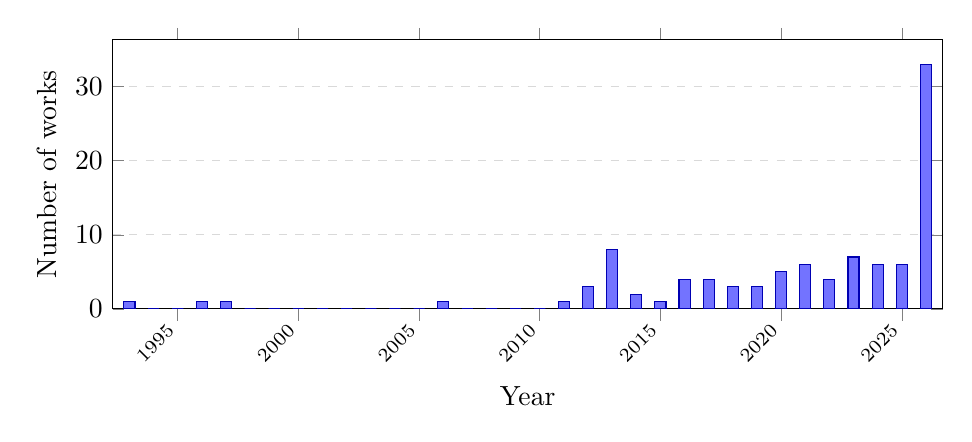
\begin{tikzpicture}
\begin{axis}[
  ybar, width=\columnwidth, height=5cm, bar width=4pt,
  xmin=1992.3, xmax=2026.7, ymin=0,
  xlabel={Year}, ylabel={Number of works},
  xtick distance=5, x tick label style={/pgf/number format/1000 sep=, rotate=45, anchor=east, font=\scriptsize},
  ymajorgrids, grid style={dashed,gray!30}, enlarge x limits=false]
\addplot[fill=blue!55, draw=blue!70!black] coordinates {(1993,1) (1994,0) (1995,0) (1996,1) (1997,1) (1998,0) (1999,0) (2000,0) (2001,0) (2002,0) (2003,0) (2004,0) (2005,0) (2006,1) (2007,0) (2008,0) (2009,0) (2010,0) (2011,1) (2012,3) (2013,8) (2014,2) (2015,1) (2016,4) (2017,4) (2018,3) (2019,3) (2020,5) (2021,6) (2022,4) (2023,7) (2024,6) (2025,6) (2026,33)};
\end{axis}
\end{tikzpicture}
\caption{Distribution of the surveyed works by publication year.}
\label{fig:years}
\end{figure}
\subsection{Cross-Cutting Trends in the Literature}
The temporal distribution of the surveyed literature, summarized in Fig.~\ref{fig:years}, spans more than three decades (1993--2026) and reveals a markedly non-uniform growth pattern: foundational theoretical contributions from the 1990s and 2000s \cite{dagum1993approximating,zhang1996exploiting,tsamardinos2006max} are followed by a long period of steady methodological consolidation, before an sharp acceleration in the last three years, which account for 45\% of the 100 works reviewed and a peak in 2026. This recent surge is dominated by applications of dynamic and causal Bayesian networks to streaming, temporal, and high-dimensional data \cite{zhang2026causal,zhang2026causalb,zhang2026causalc,zhang2026causalk,zhang2026causall,zhang2026causalr,zhang2026causals}, as well as by hybridizations with neural, symbolic, and quantum-inspired paradigms \cite{zhang2026causalo,zhang2026adaptive,zhang2026quantum,zhang2026neuro}. This pattern suggests that Bayesian networks, far from being a legacy formalism, are being actively repurposed as a substrate for integrating probabilistic reasoning with modern AI architectures, particularly in response to demands for interpretability and causal grounding that purely statistical deep learning models struggle to satisfy \cite{gao2026bayesian,geetha2023understanding,revista2026network}.

\subsection{Convergence of Causal Discovery and Deep Representation Learning}
A dominant cross-cutting theme is the convergence between classical Bayesian network structure learning and deep representation learning. Early approximate-inference and structure-learning work established the algorithmic backbone---constraint-based search \cite{tsamardinos2006max,madsen2016parallel}, score-based dynamic programming \cite{singh2018finding}, integer programming \cite{cussens2017bayesian}, and MCMC-based sampling \cite{kuipers2021efficient}---which later surveys and validations systematized and benchmarked \cite{kitson2023survey,zhou2011structure,constantinou2021large,kitson2024impact}. The recent wave of causal-discovery papers builds directly on this foundation but increasingly substitutes or augments these combinatorial searches with neural components: variational inference for joint structure-and-parameter learning \cite{zhang2026causalp,zhang2026causalb}, attention-based convolutional networks for temporal causal graphs \cite{nauta2019causal}, deep Bayesian network learners \cite{zhang2026causalo}, and episodic-memory or graph-neural architectures \cite{zhang2026causalq,zhang2026graph,zhang2026graphb}. This mirrors the broader trend identified in works that explicitly bridge graphical models and neural networks for structured inference \cite{j2016composing,mnih2014neural,gal2015bayesian,mobiny2021dropconnect}, and in generative approaches to Bayesian computation \cite{polson2023generative}. Temporal extensions---dynamic Bayesian networks, Hidden Markov Model hybrids, and Granger-causality integrations \cite{zhang2026causale,zhang2026causalf,zhang2026causalm,zhang2026dynamicb,zhang2026dynamic,motzek2017indirect,liang2020dynamic,figueroa2013temporal}---constitute perhaps the single most populous sub-theme, reflecting sustained interest in modeling evolving causal structure rather than static graphs, a concern also present in metaheuristic structure-learning work targeting dynamic networks \cite{meng2024dynamic}.

\subsection{Dominant Techniques, Application Domains, and Benchmarking Practices}
Across themes, three technique families recur: (i) search-and-score or constraint-based structure learning, increasingly hybridized with metaheuristics such as genetic algorithms, pigeon- and falcon-inspired optimization, bacterial foraging, and opposition-based learning \cite{kareem2019pigeon,sun2022bayesian,sun2019hybrid,liu2022bayesian,awla2023comparative,kareem2021falcon,sun2025bayesian}; (ii) exact and approximate inference algorithms---belief propagation, expectation propagation, conditioning methods, and hybrid discrete-continuous solvers---developed primarily in the 1990s--2010s and still cited as the computational backbone for newer applications \cite{murphy2013loopy,minka2013expectation,darwiche2013conditioning,heskes2012expectation,salmeron2018review,gogate2012approximate,huang2013efficient,dagum1997optimal}; and (iii) domain-specific causal or diagnostic models, most visibly in medicine, where Bayesian and causal Bayesian networks are used for diagnosis, prognosis, and explanation \cite{zhang2026causald,zhang2026explainable,zhang2026bayesian,selvaraj2024artificial,polotskaya2024bayesian,ma2023bayesian,mclachlan2020bayesian,chen2020interpretable,rao2023medical,nicora2024bayesian}, as well as in neuroscience \cite{bielza2014bayesian}, climate science \cite{ebertuphoff2012causal}, cybersecurity \cite{zhang2017fuzzy,munozgonzalez2017efficient}, fault diagnosis \cite{chen2023fault}, judicial decision support \cite{moric2025based}, and policy-making \cite{moreira2025bayesian}. Despite this diversity of application domains, evaluation practices remain strikingly heterogeneous and often weakly standardized: many structure-learning papers rely on classical benchmark networks (e.g., well-known discrete graphs used across \cite{kitson2023survey,constantinou2021large,kitson2024impact,trosser2021improved}), while the 2026 wave of causal-discovery papers more frequently reports on synthetic or simulated streaming/time-series data with less consistent baselines, making cross-paper comparison difficult. Where human-centered evaluation is attempted, it is rare and qualitative, as in the user study of explanation understandability for Bayesian network predictions \cite{butz2022investigating} or the comparison of explainable versus black-box models for pandemic-era hospital admission prediction \cite{nicora2024bayesian}.

\subsection{Reproducibility, Tooling, and Theoretical Grounding}
Reproducibility is unevenly supported across the literature. A relatively small number of works contribute openly usable software and pedagogical infrastructure---bnstruct for structure learning with missing data \cite{franzin2016bnstruct}, RevBayes for phylogenetic graphical models \cite{hohna2016revbayes}, and OpenMarkov as a teaching platform \cite{diez2022teaching}---which stand in contrast to the majority of application papers, especially the recent causal-discovery cluster, that do not emphasize released code, data, or standardized metrics. This gap is partly mitigated by theoretical and complexity-oriented work that provides durable, reproducible guarantees independent of implementation: NP-hardness results for approximate inference \cite{dagum1993approximating}, polytope and facet analyses for optimal structure learning \cite{cussens2017bayesian}, insensitivity-to-imprecision analyses for diagnostic belief networks \cite{henrion2013why}, and missing-data handling frameworks \cite{mohan2013graphical,franzin2016bnstruct}. Large-scale empirical validations such as \cite{constantinou2021large} and comprehensive surveys \cite{kitson2023survey,zhou2011structure,salmeron2018review} play an important role in aggregating and stress-testing algorithmic claims that individual papers rarely benchmark against one another, partially compensating for the field's fragmented evaluation culture.

\subsection{Synthesis}
Taken together, the surveyed works depict Bayesian networks as a mature yet actively evolving formalism whose theoretical core---structure learning, exact/approximate inference, and causal semantics---was substantially settled between the 1990s and early 2010s \cite{dagum1993approximating,zhang1996exploiting,tsamardinos2006max,singh2018finding,murphy2013loopy,darwiche2013conditioning}, while its recent trajectory, concentrated in the last three years per Fig.~\ref{fig:years}, is defined by integration with deep learning, streaming/temporal data, and explainability demands \cite{zhang2026causal,zhang2026neuro,zhang2026adaptive,nicora2024bayesian,kim2025understanding}. The dominant open issue is not algorithmic novelty but methodological rigor: the proliferation of similarly framed dynamic/causal Bayesian network variants in 2026 outpaces the field's capacity to benchmark them against shared datasets, common baselines, or openly reproducible implementations, a concern echoed by broader reviews calling for consolidation of causal discovery and probabilistic graphical model research \cite{gao2026bayesian,revista2026network,geetha2023understanding}.

\section{Open Challenges and Future Directions}\label{sec:challenges}
\subsection{Scalability and Computational Complexity of Structure Learning}
Learning the directed acyclic graph (DAG) that best represents a domain remains one of the most persistent bottlenecks in Bayesian network research. The task is fundamentally a combinatorial optimization problem: the number of candidate DAGs grows super-exponentially with the number of variables, and the acyclicity constraint prevents the use of standard convex optimization machinery \cite{kuipers2021efficient,zhou2011structure,sun2022bayesian}. Surveys covering dozens of structure-learning algorithms confirm that no single method dominates across problem settings, and that determining graph structure under causal assumptions is especially fraught \cite{kitson2023survey}. Integer-programming formulations have improved optimality guarantees, yet foundational understanding of the polytopes underlying these approaches is still incomplete \cite{cussens2017bayesian}, and the sheer size of the search space continues to challenge even hybrid and metaheuristic solvers \cite{sun2019hybrid}. Promising directions include tighter integration of constraint propagation with optimization-based search, better theoretical characterization of search-space geometry, and further development of scalable approximate and anytime algorithms that trade optimality for tractability on high-dimensional problems.

\subsection{Tractable Exact and Approximate Inference at Scale}
Even when a correct network structure is available, inference---the computation of posterior marginals or conditional probabilities---remains provably hard: approximating conditional probabilities in belief networks is NP-hard, just as exact inference is \cite{dagum1993approximating}. Loopy belief propagation and related message-passing schemes offer practical approximations, but their behavior is unpredictable: empirical studies show convergence and good accuracy on some real-world networks while exhibiting oscillation and no clear relationship to correct posteriors on others \cite{murphy2013loopy}. Expectation propagation partially generalizes belief propagation to hybrid discrete-continuous settings, yet it remains best suited to restricted classes of networks and lacks guaranteed closed-form solutions in general hybrid models \cite{minka2013expectation,salmeron2018review}. Applications such as attack-graph analysis further illustrate that exact inference simply does not scale to realistic problem sizes, forcing reliance on approximate methods whose error behavior is not well characterized \cite{munozgonzalez2017efficient,gogate2012approximate}. Future work should prioritize inference algorithms with provable convergence and error bounds for hybrid and loopy structures, along with principled criteria for predicting when approximate methods will fail before deployment.

\subsection{Causal Discovery from Dynamic, Streaming, and Temporal Data}
A large and rapidly growing body of work seeks to extend Bayesian networks beyond static, fully observed snapshots toward settings where data arrives continuously or evolves over time. Traditional causal discovery methods assume access to a complete dataset, a constraint that severely limits applicability in dynamic, evolving environments \cite{zhang2026dynamic}, and conventional algorithms similarly struggle to capture complex temporal dependencies, limiting their interpretability and predictive accuracy \cite{zhang2026dynamicc}. Proposed remedies include dynamic structure-learning algorithms that continuously update topology and parameters as new data arrive \cite{zhang2026causal,zhang2026causalb}, Bayesian inference frameworks explicitly designed to mitigate confounding and model temporal dependence \cite{zhang2026causalc}, integration with Hidden Markov Models to represent latent temporal states \cite{zhang2026causalf,zhang2026causale}, and intervention-aware or MCMC-based dynamic Bayesian network formulations tailored to streaming and intervention-laden data \cite{zhang2026dynamicb,zhang2026causall,zhang2026causalr,zhang2026causals,zhang2026causali}. High-dimensional time series pose additional difficulty, as causal relationships must be disentangled from confounding and intricate temporal structure simultaneously \cite{zhang2026causalk}, and nature-inspired optimization has been proposed to improve dynamic structure search \cite{meng2024dynamic}. Because most of these proposals remain theoretical or conceptual frameworks awaiting empirical validation, a key open direction is rigorous benchmarking of dynamic and streaming causal discovery methods against realistic, non-stationary data-generating processes.

\subsection{Latent Confounders, Feedback Loops, and Violations of Causal Sufficiency}
Standard causal discovery algorithms typically assume causal sufficiency---that no unmeasured confounder influences multiple observed variables---and acyclicity of the underlying graph, assumptions that are routinely violated in practice. Work on dynamic Bayesian networks explicitly acknowledges that latent variables and feedback loops complicate causal discovery and require dedicated modeling machinery rather than being treated as noise \cite{zhang2026causale}. Confounding factors intertwined with temporal dependencies are similarly flagged as a core obstacle to reliable causal inference from time-varying data \cite{zhang2026causalc}. More broadly, large-scale empirical validation shows that structure-learning algorithms are typically developed and evaluated under assumptions of complete data and causal sufficiency that are unrealistic in real-world deployments, meaning synthetic benchmark performance likely overestimates real-world performance to an unknown degree \cite{constantinou2021large}. Addressing this gap calls for structure-learning methods that explicitly model latent confounding (e.g., via latent-variable DAGs or ancestral graphs), feedback-aware extensions of dynamic Bayesian networks, and evaluation protocols using data that deliberately violate idealized assumptions so that robustness, not just accuracy under ideal conditions, can be measured.

\subsection{Robustness to Missing, Noisy, and Non-Ideal Data}
Real-world datasets are rarely complete, yet most structure-learning theory is developed under an implicit assumption of fully observed data. Tools such as bnstruct were developed specifically because, to the best of the authors' knowledge, no other open-source software jointly supported structure learning, parameter learning, and inference in the presence of missing values \cite{franzin2016bnstruct}, underscoring how underserved this problem has been at the tooling level. On the theoretical side, graphical-model-based procedures have been shown to overcome limitations of conventional missing-data methods and to provide performance guarantees even under Missing Not At Random (MNAR) mechanisms \cite{mohan2013graphical}, yet such guarantees are not uniformly available across algorithm families. Compounding this, empirical validation under noisy, real-world-like data reveals that algorithm rankings and performance can diverge substantially from idealized benchmarks \cite{constantinou2021large}. Future research should focus on extending missing-data-aware inference and learning theory to a broader range of structure-learning algorithms, developing standardized noisy-data benchmarks, and building accessible open-source tooling that makes robust handling of imperfect data the default rather than the exception.

\subsection{Hybrid Neuro-Symbolic Integration with Deep Learning}
A recurring theme across recent proposals is combining the pattern-recognition strength of neural networks with the structured, logical inference capabilities of Bayesian networks, precisely because neither paradigm alone suffices for complex, high-dimensional, and partially interpretable reasoning tasks. Frameworks merging neural pattern recognition with dynamic Bayesian network inference are explicitly motivated by the limitations of purely data-driven or purely rule-based diagnostic methods \cite{zhang2026neuro}. Similarly, graph-based reasoning combined with Bayesian network principles has been proposed to iteratively refine causal graph structure while enforcing consistency constraints, with explicit calls for future work combining such hybrids with reinforcement learning and domain knowledge \cite{zhang2026graph}. Deep neural networks have also been proposed to directly learn conditional independence structure from data, moving beyond strong parametric assumptions or reliance on expert knowledge \cite{zhang2026causalo}, while symbolic reasoning engines have been integrated with data-driven causal discovery specifically to curb spurious correlations and restore interpretability \cite{zhang2026adaptive}. Generative deep learning has further been proposed as a density-free route to Bayesian posterior computation \cite{polson2023generative}, and Bayesian approximations such as DropConnect illustrate the broader push to equip deep networks with calibrated

\section{Conclusion}\label{sec:conclusion}
Bayesian networks have evolved from a formalism for compact probabilistic representation into a central methodological bridge connecting statistical inference, causal reasoning, and modern AI systems. The taxonomy developed in this survey organizes the literature into seven interrelated strands: causal discovery from observational and streaming data, the integration of probabilistic graphical models within broader AI architectures, causal Bayesian networks for medical decision-making, the foundational problems of structure learning and conditional independence testing, exact and approximate inference algorithms, metaheuristic approaches to structure optimization, and the computational complexity results that bound what is achievable in all of the above. Across these strands, a consistent pattern emerges: the field has progressively moved from static, hand-specified networks toward dynamic, data-driven, and hybrid neuro-probabilistic models, exemplified by dynamic Bayesian network formulations for streaming and time-series causal discovery \cite{zhang2026causal,zhang2026causalb,zhang2026causalc,zhang2026dynamic} and by architectures that fuse graphical models with neural components for scalable inference and representation learning \cite{j2016composing,mnih2014neural,polson2023generative}. At the same time, classical contributions on structure learning algorithms, conditional independence foundations, and exact/approximate inference \cite{kitson2023survey,kuipers2021efficient,tsamardinos2006max,murphy2013loopy,darwiche2013conditioning,minka2013expectation,zhang1996exploiting} remain the backbone upon which these newer developments are built, while metaheuristic optimization techniques such as genetic algorithms, pigeon-inspired optimization, and hybrid swarm methods \cite{kareem2019pigeon,sun2022bayesian,sun2019hybrid,liu2022bayesian,sun2025bayesian} offer practical means of navigating the combinatorially vast space of candidate network structures.

A central finding is that the appeal of Bayesian networks lies in their dual capacity to support both predictive inference and causal explanation, a property that has made them especially prominent in high-stakes, interpretability-sensitive domains such as medical diagnosis, where causal Bayesian networks are used to model symptom-disease-treatment pathways and to generate human-interpretable explanations of AI predictions \cite{zhang2026causald,zhang2026explainable,zhang2026bayesian,amato2013artificial,butz2022investigating}. This interpretability, however, is counterbalanced by fundamental computational limits: exact inference and even approximate inference in general Bayesian networks are provably intractable in the worst case \cite{dagum1993approximating}, and optimal structure learning is similarly hard, as formalized through dynamic programming and integer programming analyses of the search space \cite{singh2018finding,cussens2017bayesian}. Reviews and surveys of structure learning and of the broader probabilistic graphical model landscape \cite{kitson2023survey,zhou2011structure,gao2026bayesian,revista2026network} confirm that no single algorithmic paradigm dominates; rather, practitioners must trade off accuracy, scalability, and robustness to missing or noisy data \cite{franzin2016bnstruct,mohan2013graphical} depending on application constraints, as also illustrated by decision-theoretic and autonomous-systems use cases \cite{abdallah2025advancing,zhang2026causalg,vargasserna2025neural}.

Looking forward, the most pressing directions concern reconciling the scalability demands of modern AI with the interpretability and causal rig

\bibliographystyle{IEEEtran}
\bibliography{refs}
\end{document}
